\chapter{Desarrollo e implementación \newline (Segunda iteración)}\label{ch:conclusiones-trabajo-a-futuro}
Este capítulo describe el proceso completo de desarrollo e implementación del sistema. Se detalla la arquitectura del sistema, el desarrollo del backend y frontend, la estructura de datos utilizada, el análisis de eficiencia algorítmica, así como el despliegue en un entorno de servidor. Además, se incluyen las pruebas realizadas para validar el funcionamiento y rendimiento del sistema, junto con consideraciones de seguridad y escalabilidad. Este capítulo representa el núcleo técnico del proyecto, integrando tanto los aspectos computacionales como los educativos.

\section{Desarrollo del Backend}
\label{sec:backend-desarrollo}

El backend de la aplicación fue desarrollado utilizando \textbf{Node.js} con el framework \textbf{Express.js}, y constituye el motor computacional encargado del procesamiento simbólico de las series de Fourier. Este componente se comunica directamente con el sistema de álgebra computacional \textbf{Maxima}, ejecutando scripts generados dinámicamente para realizar integración simbólica, manipulación de expresiones y evaluación de límites. Su diseño modular y jerarquizado permite separar con claridad las capas de comunicación HTTP, lógica de negocio, procesamiento utilitario y sistemas externos.

\subsection{Arquitectura en Capas}

El backend está estructurado bajo un patrón de arquitectura en capas, con el objetivo de asegurar mantenibilidad, extensibilidad y separación de responsabilidades. Las capas principales son:

\begin{itemize}
	\item \textbf{Capa HTTP (Controladores)}: expone la interfaz RESTful mediante Express, manejando rutas como \texttt{/api/fourier-series/*}. Esta capa recibe solicitudes, extrae parámetros, valida datos y delega el cálculo a la capa de servicios.
	
	\item \textbf{Capa de Servicios}: encapsula la lógica principal para el cálculo de series de Fourier en sus distintas variantes (trigonométricas, exponenciales complejas, de medio rango, y transformadas discretas). Se apoya en funciones auxiliares para validaciones, construcción de scripts y análisis de singularidades.
	
	\item \textbf{Capa Utilitaria}: agrupa funciones para la validación matemática, generación de scripts Maxima, manejo de funciones por tramos y reglas de simplificación.
	
	\item \textbf{Sistema Externo}: corresponde al motor simbólico \textbf{Maxima}, invocado a través de la línea de comandos desde Node.js mediante \texttt{child\_process.exec}.
\end{itemize}

\begin{figure}[H]
	\centering
	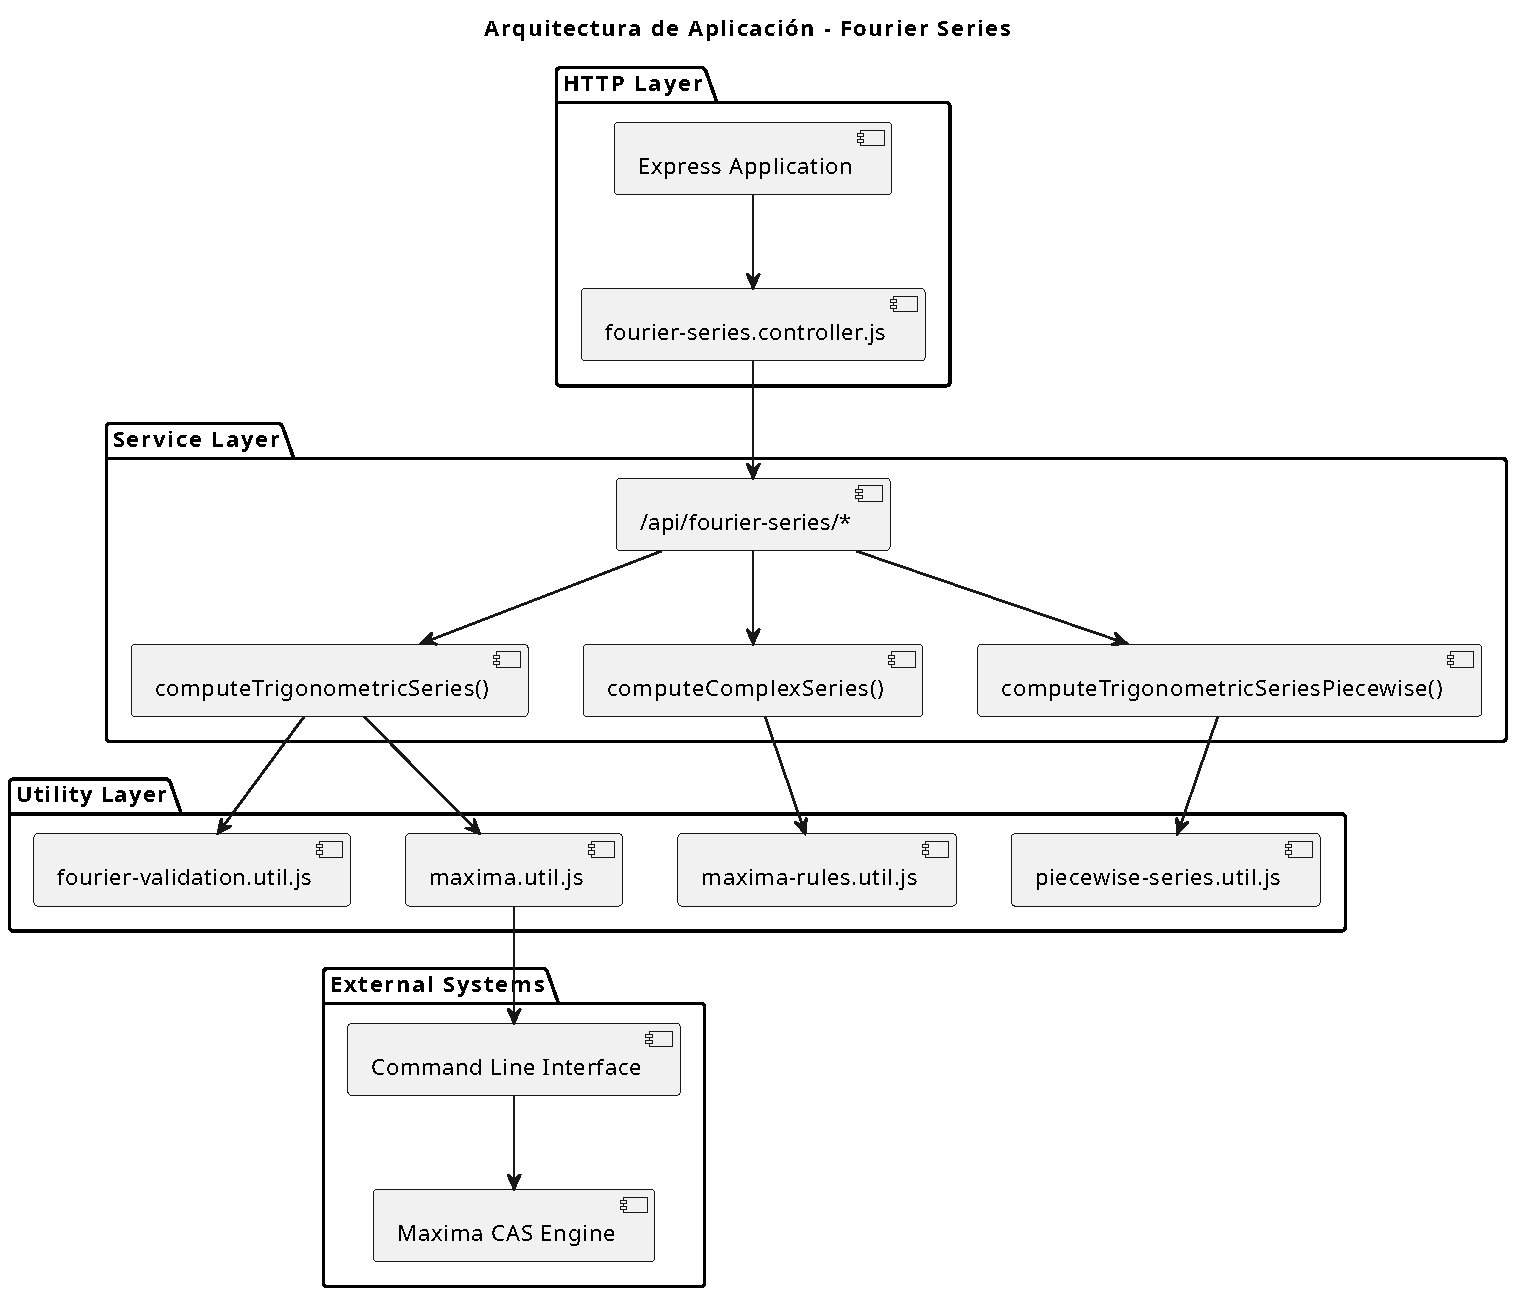
\includegraphics[width=1\textwidth]{img/chapter07/arqui-apliacion.pdf}
	\caption[Arquitectura modular del backend para el cálculo de series de Fourier.]{Arquitectura modular del backend para el cálculo de series de Fourier. \textit{Fuente: \textit{Elaboración propia}}}
	\label{fig:backend-architecture}
\end{figure}

\subsection{Controladores y Endpoints}

La capa de controladores está centralizada en el archivo \texttt{fourier-series.controller.js}, donde se definen los siguientes endpoints:

\begin{itemize}
	\item \texttt{POST /fourier-series/trigonometric-piecewise}
	\item \texttt{POST /fourier-series/complex-piecewise}
	\item \texttt{POST /fourier-series/half-range}
	\item \texttt{POST /dft/calculate}
	\item \texttt{POST /series-expansion/\{type\}}
\end{itemize}

Cada uno de estos controladores implementa un patrón uniforme: 
1) extracción de parámetros desde el cuerpo de la solicitud, 
2) validación matemática simbólica de las expresiones, 
3) invocación del motor de cálculo, 
4) gestión de errores, y 
5) construcción de la respuesta con expresiones en notación simbólica y LaTeX.

\subsection{Integración con Maxima}

La integración con Maxima se realiza mediante scripts generados dinámicamente a partir de las entradas del usuario. Estos scripts contienen definiciones de las funciones por tramos, declaraciones de variables simbólicas, reglas de simplificación, y comandos de integración.

La función \texttt{calculatePiecewiseSeries()} orquesta el proceso de cálculo, diferenciando entre tipos de serie mediante lógica condicional y asegurando que cada tipo se procese con su núcleo de integración correspondiente. Se ejecutan tres fases:
\begin{enumerate}
	\item Cálculo simbólico sin restricción de $n$ entero.
	\item Detección de indeterminaciones mediante resolución de ecuaciones sobre denominadores.
	\item Cálculo final con $n \in \mathbb{Z}$ y resolución de límites en los casos necesarios.
\end{enumerate}

Estas fases permiten generar resultados consistentes incluso en presencia de formas indeterminadas del tipo $\frac{0}{0}$. Se utiliza \texttt{Promise.all} para ejecutar múltiples tareas de cálculo en paralelo, optimizando tiempos de respuesta.

\subsection{Sistema de Validación Matemática}

La validación previa al cálculo simbólico es realizada por el módulo \texttt{fourier-validation.util.js}, que implementa funciones como:

\begin{itemize}
	\item \texttt{validateIntegrability(func, intVar, a, b, kernel)}: verifica que las integrales de los coeficientes sean computables simbólicamente.
	\item \texttt{validateFourierSeries(options)}: valida series simples.
	\item \texttt{validatePiecewiseFourierSeries(funcionMatrix, intVar, type)}: analiza la integrabilidad de cada tramo de forma independiente.
\end{itemize}

En caso de que alguna validación falle, el sistema responde con un código HTTP \texttt{422 Unprocessable Entity} y un objeto estructurado que detalla qué coeficientes no pueden integrarse, y si se detectaron funciones especiales.

\subsection{Estructura de Datos y Formato de Respuesta}

La comunicación entre cliente y servidor se realiza mediante objetos JSON. Las solicitudes para funciones por tramos siguen la siguiente estructura:


\begin{listing}[H] % requiere \usepackage{float}
\begin{minted}[fontsize=\small, linenos, breaklines]{json}
		{
			"funcionMatrix": [
			["x^2", "0", "1"],
			["sin(x)", "1", "2"]
			],
			"intVar": "x"
		}
	\end{minted}
	\caption{DTO de entrada para series por tramos}
	\label{lst:piecewise-request}
\end{listing}

Las respuestas exitosas contienen expresiones simbólicas simplificadas, representaciones LaTeX, valores de $T$, $\omega_0$ y detección de valores indeterminados, como se muestra a continuación:

\begin{listing}[H]
\begin{minted}[fontsize=\small, linenos, breaklines]{json}
		{
			"success": true,
			"simplified": {
				"a0": "expression",
				"an": "expression",
				"bn": "expression",
				"T": "2",
				"w0": "pi"
			},
			"latex": {
				"a0": "LaTeX_a0",
				"an": "LaTeX_an",
				"bn": "LaTeX_bn"
			},
			"indeterminateValues": {
				"an": [{ "n": 2, "limit": "0", "limitTex": "0" }]
			}
		}
	\end{minted}
	\caption{DTO de salida para serie trigonométrica por tramos}
	\label{lst:piecewise-response}
\end{listing}

\subsection{Transformada Discreta de Fourier (DFT)}

El sistema también incluye un endpoint dedicado para calcular la \textbf{Transformada Discreta de Fourier (DFT)} de funciones definidas por tramos. Esta funcionalidad permite analizar espectros de frecuencia mediante muestreo simbólico, y se integra en la misma arquitectura modular del backend.

\subsubsection*{DTO de Solicitud para DFT}

La petición al endpoint de DFT requiere una estructura JSON con los siguientes parámetros:

\begin{listing}[H]
	\begin{minted}[fontsize=\small, linenos, breaklines]{json}
		{
			"funcionMatrix": [
			["sin(x)", "0", "pi"],
			["0", "pi", "2*pi"]
			],
			"N": 128,
			"M": 2,
			"intVar": "x"
		}
	\end{minted}
	\caption{DTO de entrada para cálculo de DFT}
	\label{lst:dft-request}
\end{listing}

\begin{itemize}
	\item \texttt{funcionMatrix}: matriz de definición por tramos.
	\item \texttt{N}: número de puntos de muestreo.
	\item \texttt{M}: factor de extensión del dominio para graficación.
	\item \texttt{intVar}: variable de integración (generalmente \texttt{"x"} o \texttt{"t"}).
\end{itemize}

\subsubsection*{DTO de Respuesta para DFT}

La respuesta del backend incluye los datos necesarios para visualizar la señal reconstruida, junto con su espectro de frecuencia en términos de amplitud y fase:

\begin{listing}[H]
	\begin{minted}[fontsize=\small, linenos, breaklines]{json}
		{
			"success": true,
			"data": "[0.0, 0.5, 1.0, ...]",
			"originalPoints": "[0.0, 1.0, 0.0, ...]",
			"amplitudeSpectrum": "[[0, 1.0], [1, 0.5], ...]",
			"phaseSpectrum": "[[0, 0], [1, -1.57], ...]"
		}
	\end{minted}
	\caption{DTO de salida para resultado de DFT}
	\label{lst:dft-response}
\end{listing}

\begin{itemize}
	\item \texttt{data}: puntos reconstruidos de la señal periódica.
	\item \texttt{originalPoints}: valores muestreados originalmente.
	\item \texttt{amplitudeSpectrum}: pares frecuencia–amplitud.
	\item \texttt{phaseSpectrum}: pares frecuencia–fase (en radianes).
\end{itemize}

\subsubsection*{Flujo Interno}

La lógica de cálculo para la DFT reside en un servicio especializado que genera los scripts de Maxima para evaluar las muestras de la función, aplicar la fórmula discreta y construir los espectros simbólicamente. El resultado es serializado en formato JSON y enviado al frontend, donde es interpretado y visualizado en un lienzo dedicado.


\subsection{Flujo de Procesamiento}

El flujo interno de cálculo se representa mediante el siguiente diagrama de secuencia, el cual ilustra los pasos desde la recepción de una solicitud hasta la entrega de resultados simbólicos:


\begin{figure}[H]
	\centering
	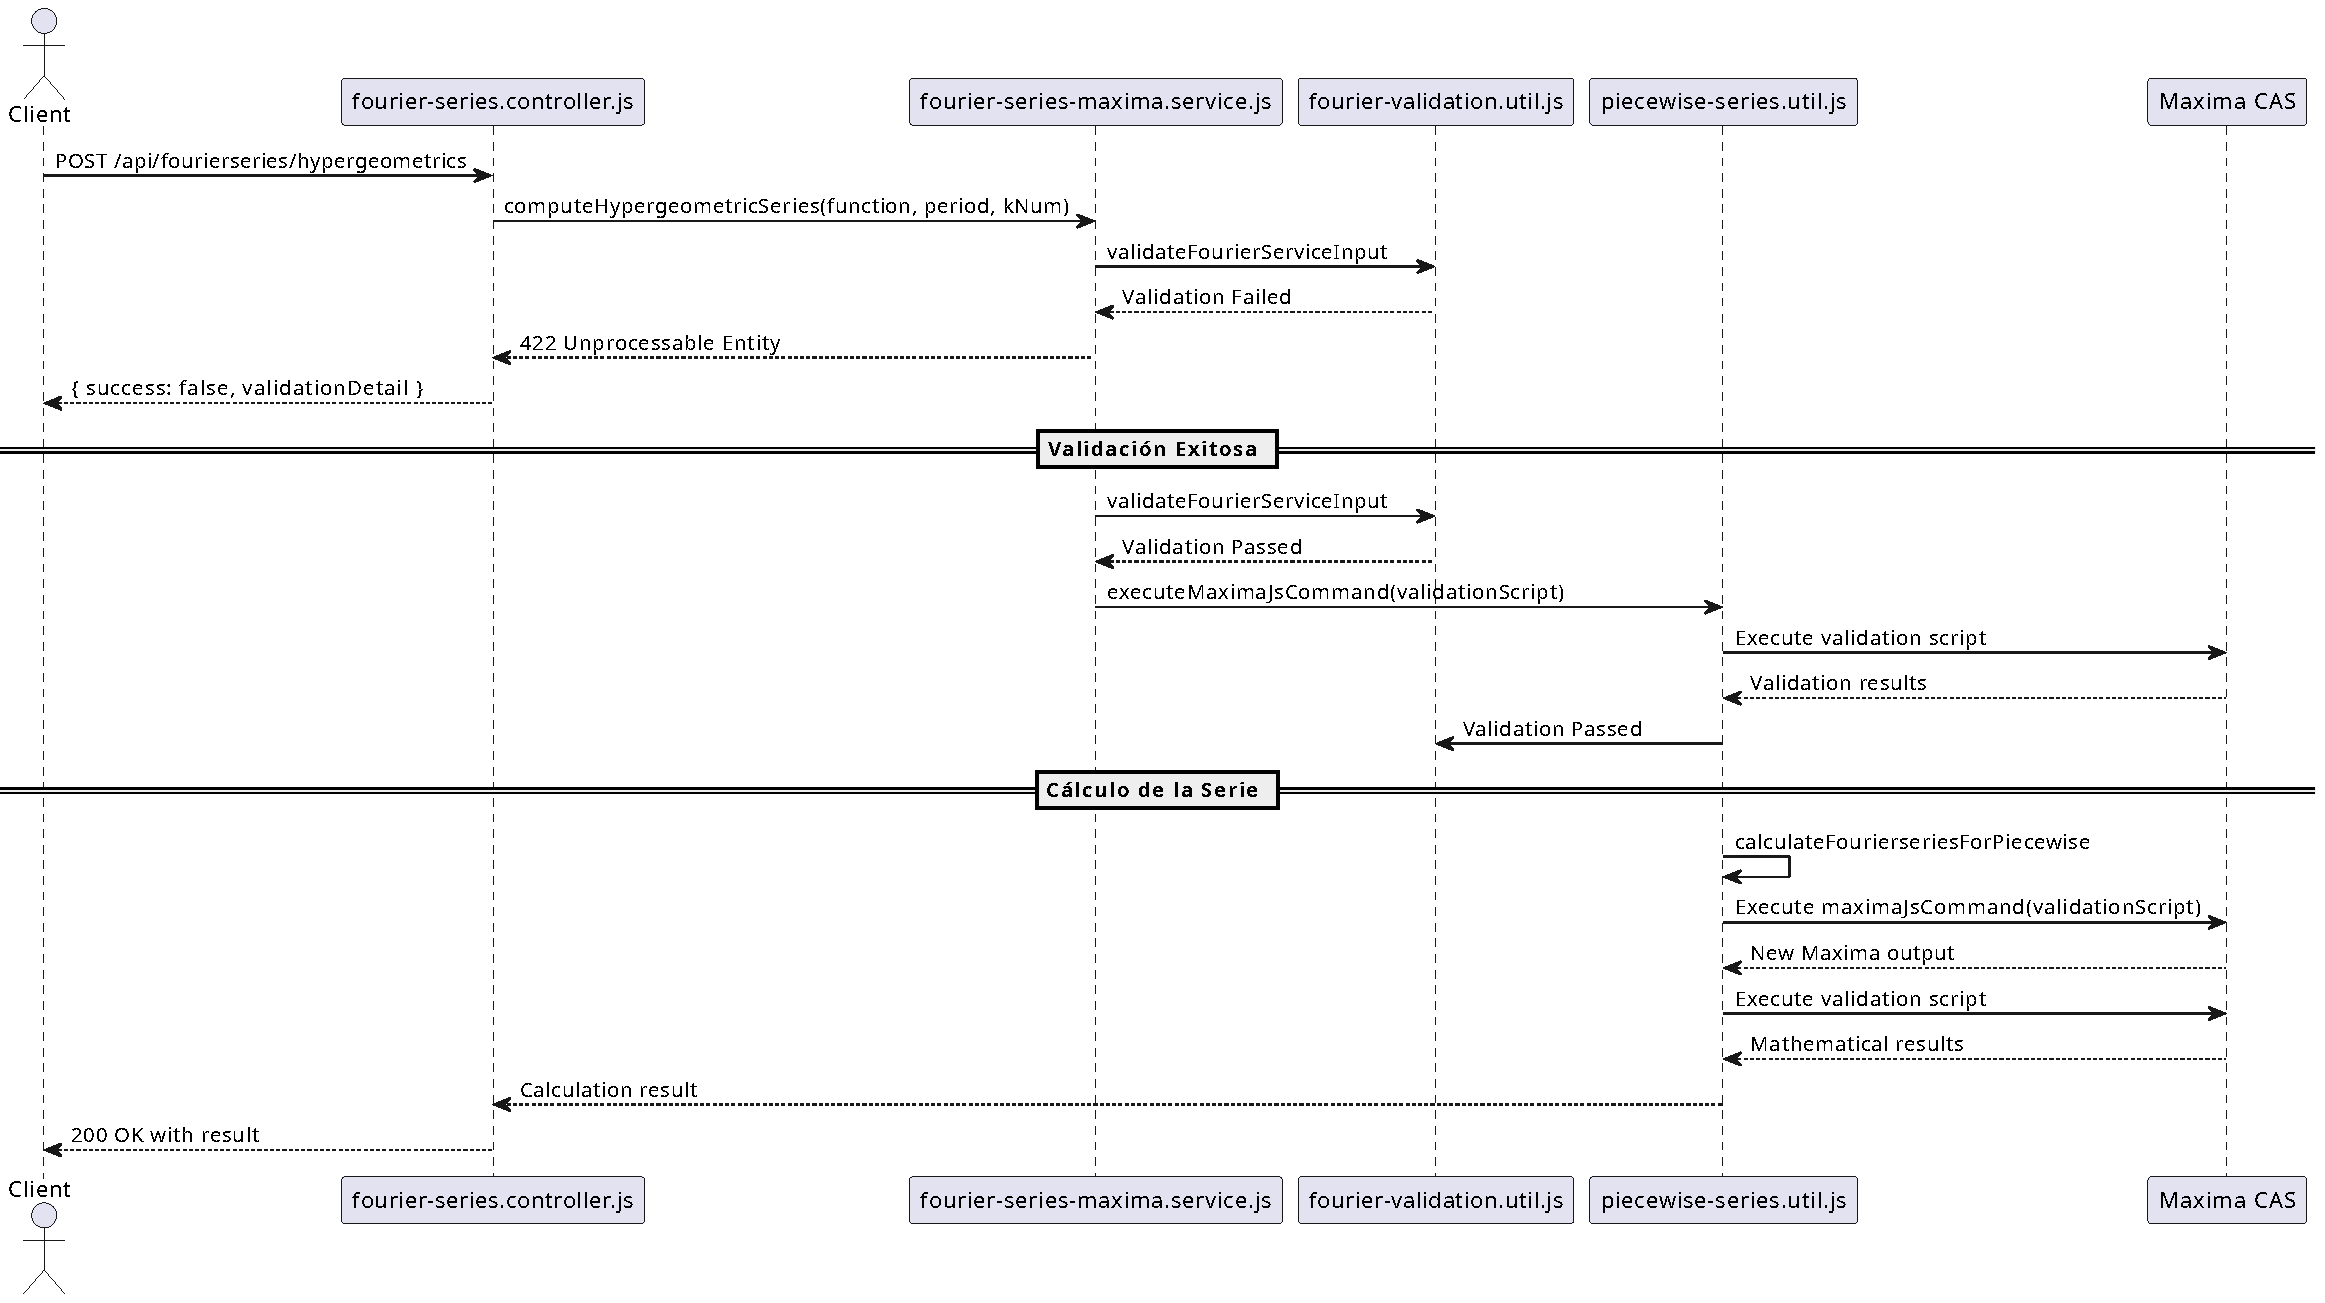
\includegraphics[width=1\textwidth]{img/chapter07/secuencia-back.pdf}
	\caption[Flujo de procesamiento interno para el cálculo de una serie de Fourier.]{Flujo de procesamiento interno para el cálculo de una serie de Fourier. \textit{Fuente: \textit{Elaboración propia}}}
	\label{fig:backend-flow}
\end{figure}



Cada componente cumple un rol específico en la cadena:
- El controlador enruta y valida.
- El servicio coordina las llamadas utilitarias.
- Los módulos de validación analizan integrabilidad.
- Maxima realiza el cálculo simbólico.
- El resultado es formateado y devuelto al cliente.

\subsection{Manejo de Errores}

El backend implementa un manejo robusto de errores con diferenciación entre fallos de validación y errores de ejecución simbólica. Se utilizan funciones auxiliares para detectar patrones de error en la salida de Maxima (\texttt{containsError}) y para extraer mensajes legibles para el usuario (\texttt{extractErrorMessage}). De esta forma, se garantiza una retroalimentación informativa y estructurada ante fallos.

\subsection{Limitaciones Técnicas}
El sistema actual presenta algunas restricciones que deben ser consideradas:

\begin{itemize}
	\item \textbf{Dependencia de sistema operativo}: la ejecución de Maxima vía línea de comandos requiere un entorno Linux para funcionar de manera estable.
	\item \textbf{Complejidad computacional}: ciertas funciones simbólicas complejas pueden producir tiempos de ejecución altos o no resolverse analíticamente.
	\item \textbf{Funciones especiales}: expresiones que involucren funciones como \texttt{erf}, \texttt{gamma} o funciones de Bessel podrían no integrarse en forma cerrada, generando errores de validación.
\end{itemize}

\subsection{Análisis de Complejidad Algorítmica}
Se realiza un análisis Big-O de los algoritmos empleados para el cálculo de series de Fourier y transformadas, considerando su comportamiento en distintos escenarios.

\section{Desarrollo del Frontend}
\label{sec:frontend-desarrollo}

El frontend de la aplicación fue desarrollado utilizando el framework \textbf{Angular 18}, junto con \textbf{TypeScript} y \textbf{TailwindCSS} para un diseño moderno, responsivo y accesible. Su objetivo es ofrecer una experiencia educativa intuitiva para definir funciones matemáticas, configurar parámetros y visualizar series de Fourier.

\subsection{Arquitectura General}

La interfaz sigue una arquitectura basada en componentes reutilizables y servicios especializados. El flujo comienza en el \texttt{HomeComponent}, encargado de la navegación inicial y ejemplos precargados. Posteriormente, se accede al \texttt{FourierCalculatorComponent}, donde el usuario define la función por tramos y selecciona el tipo de serie. Finalmente, se redirige a un componente de visualización específico para mostrar los resultados.

\begin{itemize}
	\item \textbf{Angular 18}: marco de trabajo principal con soporte para renderizado del lado servidor.
	\item \textbf{TailwindCSS}: sistema de diseño utilitario para interfaces adaptables.
	\item \textbf{MathQuill}: entrada estructurada de expresiones matemáticas.
	\item \textbf{MathJax}: renderizado de expresiones LaTeX.
	\item \textbf{Canvas personalizado}: visualización gráfica de resultados simbólicos.
\end{itemize}

\subsection{Interfaz de Entrada de Funciones}

El componente \texttt{FourierCalculatorComponent} permite la definición de funciones por tramos. Cada segmento incluye:

\begin{enumerate}
	\item Campo para la expresión simbólica (\texttt{funcField}).
	\item Intervalo inicial y final del tramo (\texttt{startField}, \texttt{endField}).
	\item Botones para agregar o eliminar segmentos.
\end{enumerate}

Cada campo se implementa como una instancia de \texttt{MathQuill}, lo que proporciona una experiencia fluida tanto en escritorio como en móviles.

\begin{figure}[H]
	\centering
	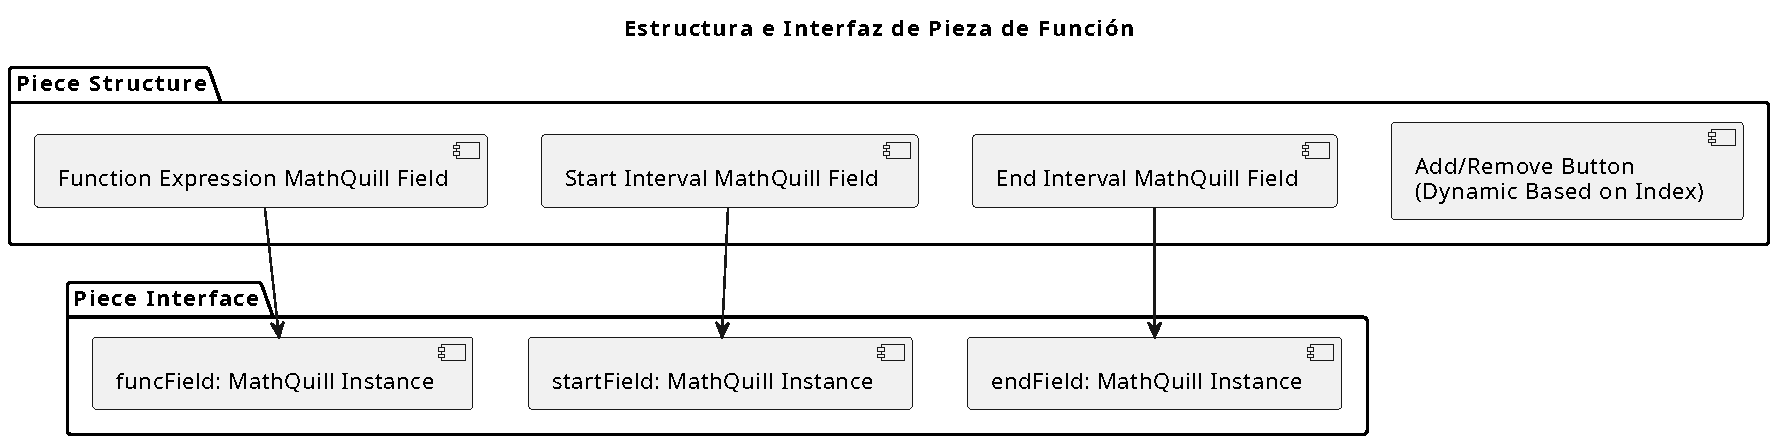
\includegraphics[width=0.75\textwidth]{img/chapter07/pieces.pdf}
	\caption[Estructura interna de los campos por tramo.]{Estructura interna de los campos por tramo. \textit{Fuente: Elaboración propia.}}
	\label{fig:frontend-piece-input}
\end{figure}

\subsection{Soporte Móvil y Teclado Matemático}

Para dispositivos móviles, se desarrolló un teclado matemático virtual con pestañas para números, variables y funciones. Esto facilita la entrada simbólica sin depender de teclados físicos.

\begin{figure}[H]
	\centering
	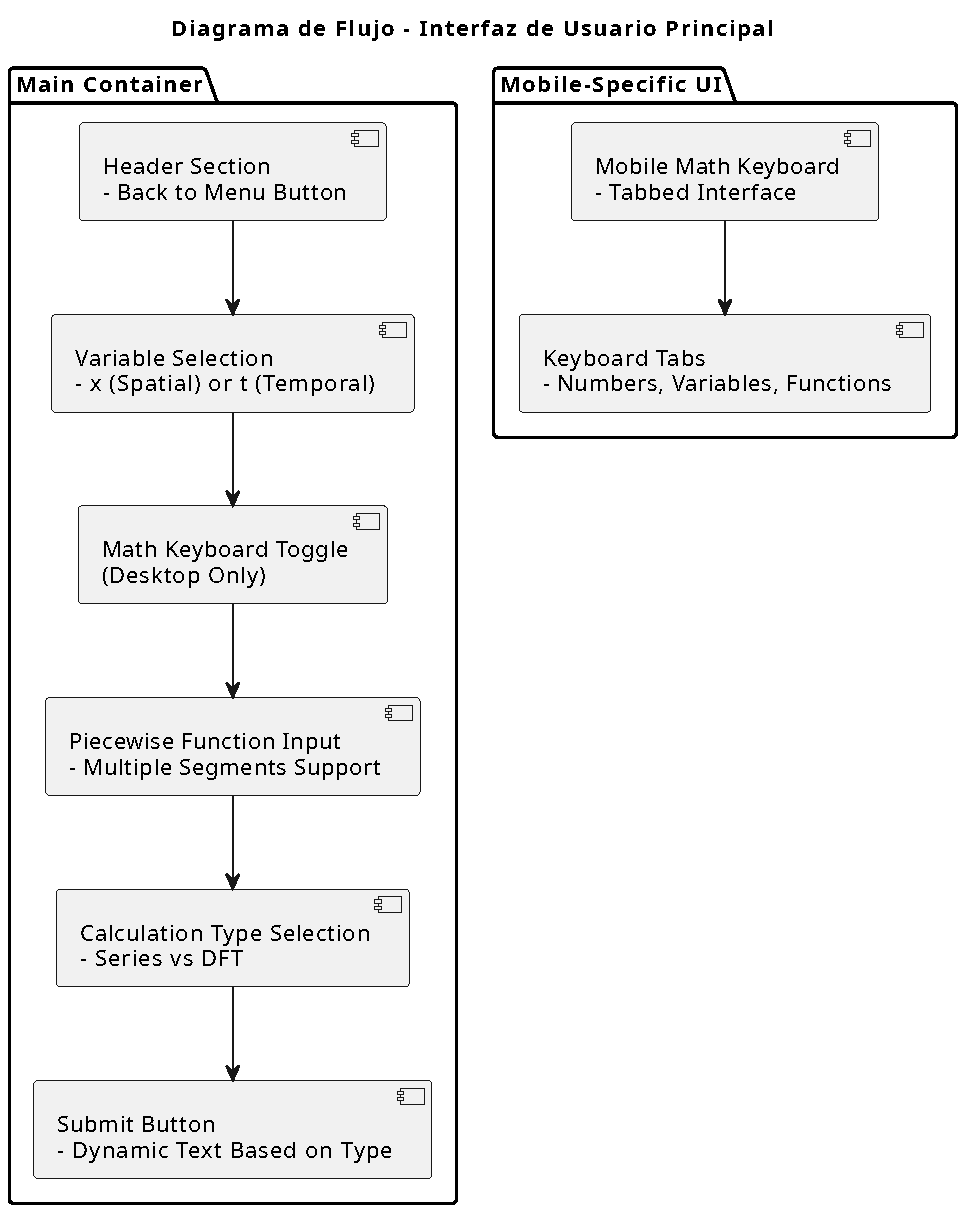
\includegraphics[width=0.8\textwidth]{img/chapter07/mobile.pdf}
	\caption[Interfaz de entrada móvil.]{Teclado matemático con pestañas: números, variables y funciones. \textit{Fuente: Elaboración propia.}}
	\label{fig:frontend-mobile-keyboard}
\end{figure}

\subsection{Visualización de Resultados}

Una vez recibida la respuesta del backend, los resultados se muestran en un componente de visualización especializado. Las fórmulas se renderizan mediante \texttt{MathJax} y las gráficas se generan sobre un lienzo interactivo:

\begin{itemize}
	\item Soporte para zoom y desplazamiento del eje.
	\item Colores diferenciados según el tipo de serie.
	\item Visualización simultánea de función original y aproximación.
	\item Ajuste dinámico del número de términos visualizados.
\end{itemize}

\subsection{Validación y Conversión de Expresiones}

Antes de enviar la solicitud, las expresiones LaTeX introducidas se convierten a sintaxis Maxima utilizando el servicio \texttt{LatexToMaximaService}. Además, se realiza una validación estructural del input:

\begin{itemize}
	\item Verificación de integridad por tramo.
	\item Detección de variables inconsistentes.
	\item Confirmación de que los campos no estén vacíos.
\end{itemize}

\subsection{Gestión de Estado y Flujo de Datos}

El sistema utiliza el \texttt{RouterState} de Angular para mantener la información entre componentes. Esto permite transiciones fluidas entre la entrada de datos y la visualización, sin pérdida de información ni recálculo.

\subsection{Rendimiento y SSR}

Se habilitó el \textbf{Server-Side Rendering (SSR)} para mejorar el tiempo de carga inicial y facilitar la indexación del contenido matemático, especialmente importante para aplicaciones educativas y accesibilidad.

\vspace{1em}

\section{Integración entre Frontend y Backend}
\label{sec:integracion-frontend-backend}

La integración entre el frontend y el backend se realiza mediante el servicio \texttt{ApiService}, que encapsula las llamadas HTTP a los distintos endpoints del servidor. Este servicio actúa como intermediario entre la entrada simbólica del usuario y el motor de cálculo basado en Maxima.

\subsection{Despacho de Cálculos y Navegación Dinámica}

Según el tipo de serie seleccionada, el frontend invoca un método específico del \texttt{ApiService}. Tras recibir una respuesta exitosa, la aplicación redirige dinámicamente al componente de visualización correspondiente, transfiriendo en el proceso el estado de cálculo (expresiones, resultados y parámetros).

\begin{itemize}
	\item \texttt{calculateTrigonometricSeriesPiecewise()} $\rightarrow$ \texttt{/fourier-series-plot/trig}
	\item \texttt{calculateComplexSeriesPiecewise()} $\rightarrow$ \texttt{/fourier-series-plot/complex}
	\item \texttt{calculateHalfRangeSeries()} $\rightarrow$ \texttt{/fourier-series-plot/half-range}
	\item \texttt{calculateDFT()} $\rightarrow$ \texttt{/fourier-transform-plot/dft}
\end{itemize}

\begin{figure}[H]
	\centering
	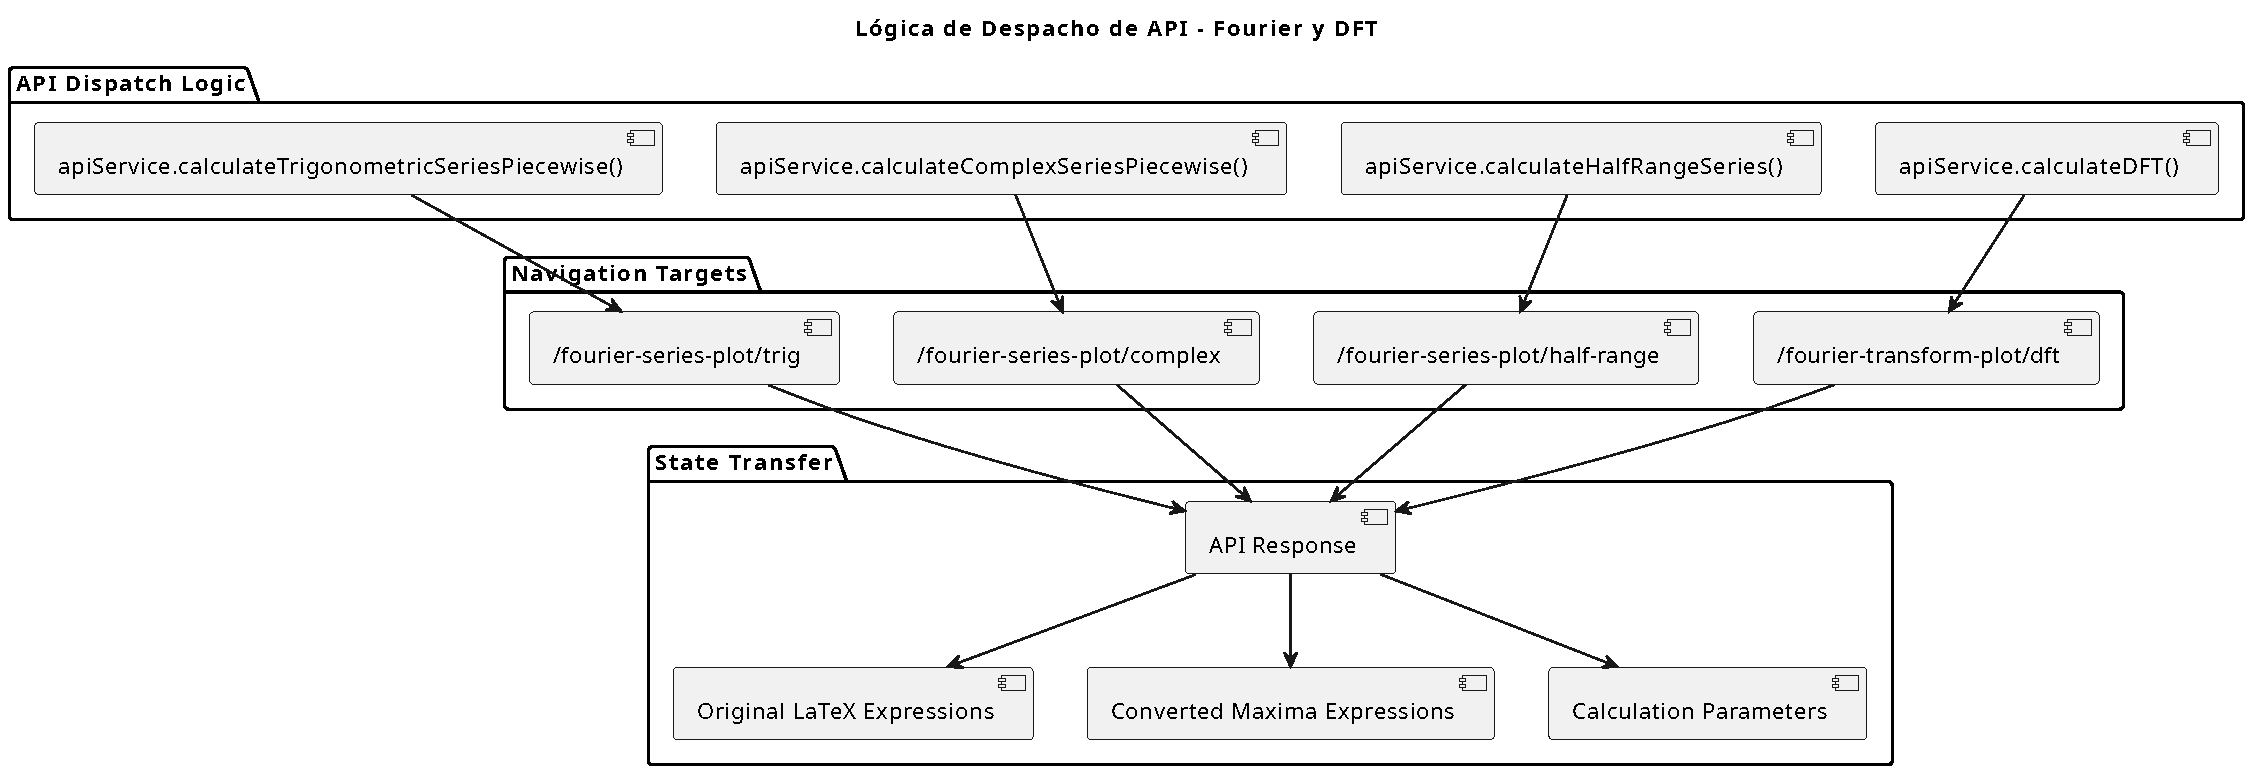
\includegraphics[width=1\textwidth]{img/chapter07/api-dispatch.pdf}
	\caption[Flujo de integración entre frontend y backend.]{Flujo de integración entre frontend y backend. \textit{Fuente: Elaboración propia.}}
	\label{fig:frontend-backend-dispatch}
\end{figure}

\subsection{Transferencia de Estado}

El sistema emplea el router de Angular con paso de parámetros en memoria. Esto permite mantener los resultados simbólicos, expresiones originales y datos intermedios entre la etapa de cálculo y la visualización sin necesidad de almacenamiento persistente.

\subsection{Manejo de Respuestas}

Las respuestas del backend incluyen:

\begin{itemize}
	\item Expresiones simbólicas simplificadas.
	\item Representación LaTeX para visualización.
	\item Valores críticos de $n$ con indeterminaciones resueltas.
	\item Información de validación y errores si corresponde.
\end{itemize}

El frontend interpreta esta información y actualiza la interfaz gráfica y simbólica según el tipo de serie.

\subsection{Robustez y Validación Cruzada}

Si el backend devuelve errores de validación (por ejemplo, funciones no integrables), el frontend responde mostrando alertas estructuradas, permitiendo al usuario corregir la entrada sin perder el progreso. Este enfoque reactivo refuerza el carácter educativo del sistema y su tolerancia a errores comunes.

\section{Despliegue y Ambientación}
\label{sec:despliegue}
Esta sección describe el proceso de publicación de la aplicación en un entorno de servidor real. Se detalla la configuración del sistema operativo, la administración de procesos de backend y frontend, y la implementación de un proxy inverso seguro mediante Nginx. Asimismo, se incluye la configuración del certificado SSL para garantizar una comunicación cifrada con los usuarios.

\subsection{Configuración del Servidor (VPS)}

La aplicación fue desplegada en un servidor privado virtual (VPS) con sistema operativo \textbf{Ubuntu Server}. Se instalaron las dependencias necesarias para la ejecución tanto del frontend como del backend, incluyendo:

\begin{itemize}
	\item Node.js (v16+) y NPM
	\item Angular CLI
	\item Maxima CAS
	\item Nginx (como servidor web)
	\item PM2 (gestor de procesos Node.js)
\end{itemize}

Tanto el frontend como el backend se ejecutan como servicios independientes sobre el mismo servidor.

\subsection{Gestión de Procesos con PM2}

Para asegurar la persistencia, monitoreo y reinicio automático de los servicios, se utilizó \textbf{PM2}. Se configuraron dos procesos principales:

\begin{itemize}
	\item \texttt{pm2 start backend}: ejecuta el servidor Express que sirve como API y conecta con Maxima.
	\item \texttt{pm2 start frontend}: ejecuta el servidor de Angular con renderizado del lado servidor (SSR) en el puerto 4000.
\end{itemize}

PM2 permite monitorear el estado de ambos procesos, reiniciarlos en caso de fallo y definir su arranque automático al iniciar el sistema operativo mediante:

\begin{minted}[fontsize=\small]{bash}
	pm2 startup
	pm2 save
\end{minted}

\subsection{Proxy Inverso con Nginx}

El acceso público a la aplicación se gestiona mediante \textbf{Nginx}, actuando como proxy inverso. Se configuraron dos bloques \texttt{upstream} para enrutar el tráfico de forma local:

\begin{itemize}
	\item \texttt{angular}: servidor frontend corriendo en el puerto \texttt{4000}.
	\item \texttt{api}: servidor backend escuchando en el puerto \texttt{3000}.
\end{itemize}

La configuración incluye una redirección automática de HTTP a HTTPS, así como reglas específicas para enrutar correctamente las rutas de API y del frontend SPA. A continuación, se presenta un fragmento del archivo de configuración de Nginx:

\begin{minted}[fontsize=\small, breaklines]{nginx}
	upstream angular {
		server 127.0.0.1:4000;
	}
	
	upstream api {
		server 127.0.0.1:3000;
	}
	
	server {
		listen 80;
		server_name fouriersolver.com www.fouriersolver.com;
		return 301 https://$host$request_uri;
	}
	
	server {
		listen 443 ssl;
		server_name fouriersolver.com www.fouriersolver.com;
		
		ssl_certificate     /etc/nginx/ssl/fouriersolver/certificado.cer;
		ssl_certificate_key /etc/nginx/ssl/fouriersolver/llave.key;
		
		ssl_protocols       TLSv1.2 TLSv1.3;
		ssl_ciphers         HIGH:!aNULL:!MD5;
		
		add_header Strict-Transport-Security "max-age=31536000; includeSubDomains" always;
		add_header X-Frame-Options DENY;
		add_header X-Content-Type-Options nosniff;
		
		location /api/ {
			proxy_pass http://api/;
			proxy_http_version 1.1;
			proxy_set_header Host $host;
			proxy_set_header X-Real-IP $remote_addr;
			proxy_set_header X-Forwarded-For $proxy_add_x_forwarded_for;
			proxy_set_header X-Forwarded-Proto $scheme;
		}
		
		location / {
			proxy_pass http://angular;
			proxy_http_version 1.1;
			proxy_set_header Host $host;
			proxy_set_header X-Real-IP $remote_addr;
			proxy_set_header X-Forwarded-For $proxy_add_x_forwarded_for;
			proxy_set_header X-Forwarded-Proto $scheme;
			
			proxy_intercept_errors on;
			error_page 404 = @rewrites;
		}
		
		location @rewrites {
			proxy_pass http://angular;
			proxy_http_version 1.1;
			proxy_set_header Host $host;
			proxy_set_header X-Real-IP $remote_addr;
			proxy_set_header X-Forwarded-For $proxy_add_x_forwarded_for;
			proxy_set_header X-Forwarded-Proto $scheme;
			
			rewrite ^ /index.html break;
		}
		
		client_max_body_size 20m;
	}
\end{minted}

\subsection{Certificado SSL}

La comunicación segura se logró mediante la instalación de un certificado digital SSL proporcionado por una autoridad certificadora. Se configuraron las siguientes rutas en el archivo de Nginx:

\begin{itemize}
	\item \texttt{/etc/nginx/ssl/fouriersolver/certificado.cer}
	\item \texttt{/etc/nginx/ssl/fouriersolver/llave.key}
\end{itemize}

Estas rutas aseguran que el sitio esté disponible bajo HTTPS, lo cual es esencial para proteger la integridad de los datos y ofrecer confianza al usuario.


%----------------------------------------------------------------------------------------
\subsection{Pruebas de Rendimiento}
El objetivo de esta campaña fue caracterizar la capacidad de respuesta y la escalabilidad
de la API bajo diferentes niveles de concurrencia.  
Para ello se utilizó Postman en modo \textit{Collection Runner} y su ejecución por línea
de comandos mediante \texttt{Newman}, lo que permitió automatizar los escenarios de carga
y capturar métricas detalladas.

\subsubsection*{Entorno de pruebas}
\begin{itemize}
	\item \textbf{Servidor de ensayo}: VPS 2\,vCore, 4 GB RAM, SSD 120 GB
	\item \textbf{Sistema operativo}: Ubuntu 22.04 LTS (64 bits)
	\item \textbf{Herramienta de carga}: Postman v10 
	\item \textbf{Escenarios}: 1 usuario virtual (1 VU) y 20 usuarios virtuales (20 VU)
\end{itemize}

\subsubsection*{Metodología}
Se ejecutaron colecciones independientes para cada uno de los cuatro endpoints críticos:

\begin{enumerate}
	\item \texttt{POST /trig-piecewise}
	\item \texttt{POST /complex-piecewise}
	\item \texttt{POST /half-range}
	\item \texttt{POST /dft}
\end{enumerate}

Cada escenario tuvo una duración fija de 60 s y se repitió tres veces, manteniendo la
misma semilla aleatoria en los cuerpos de las peticiones para favorecer la
reproducibilidad.  
Las métricas capturadas fueron:

\begin{itemize}
	\item Promedio de tiempo de respuesta (\textit{Avg. ms})
	\item Percentiles P90 y P95
	\item Solicitudes por segundo (\textit{Req/s})
	\item Tasa de error (HTTP $\ge400$)
\end{itemize}

\subsubsection*{Resultados}

%------------- 1 VU FIGURAS -------------------------------------------------
\paragraph*{Carga ligera (1 VU)}

\begin{figure}[H]
	\centering
	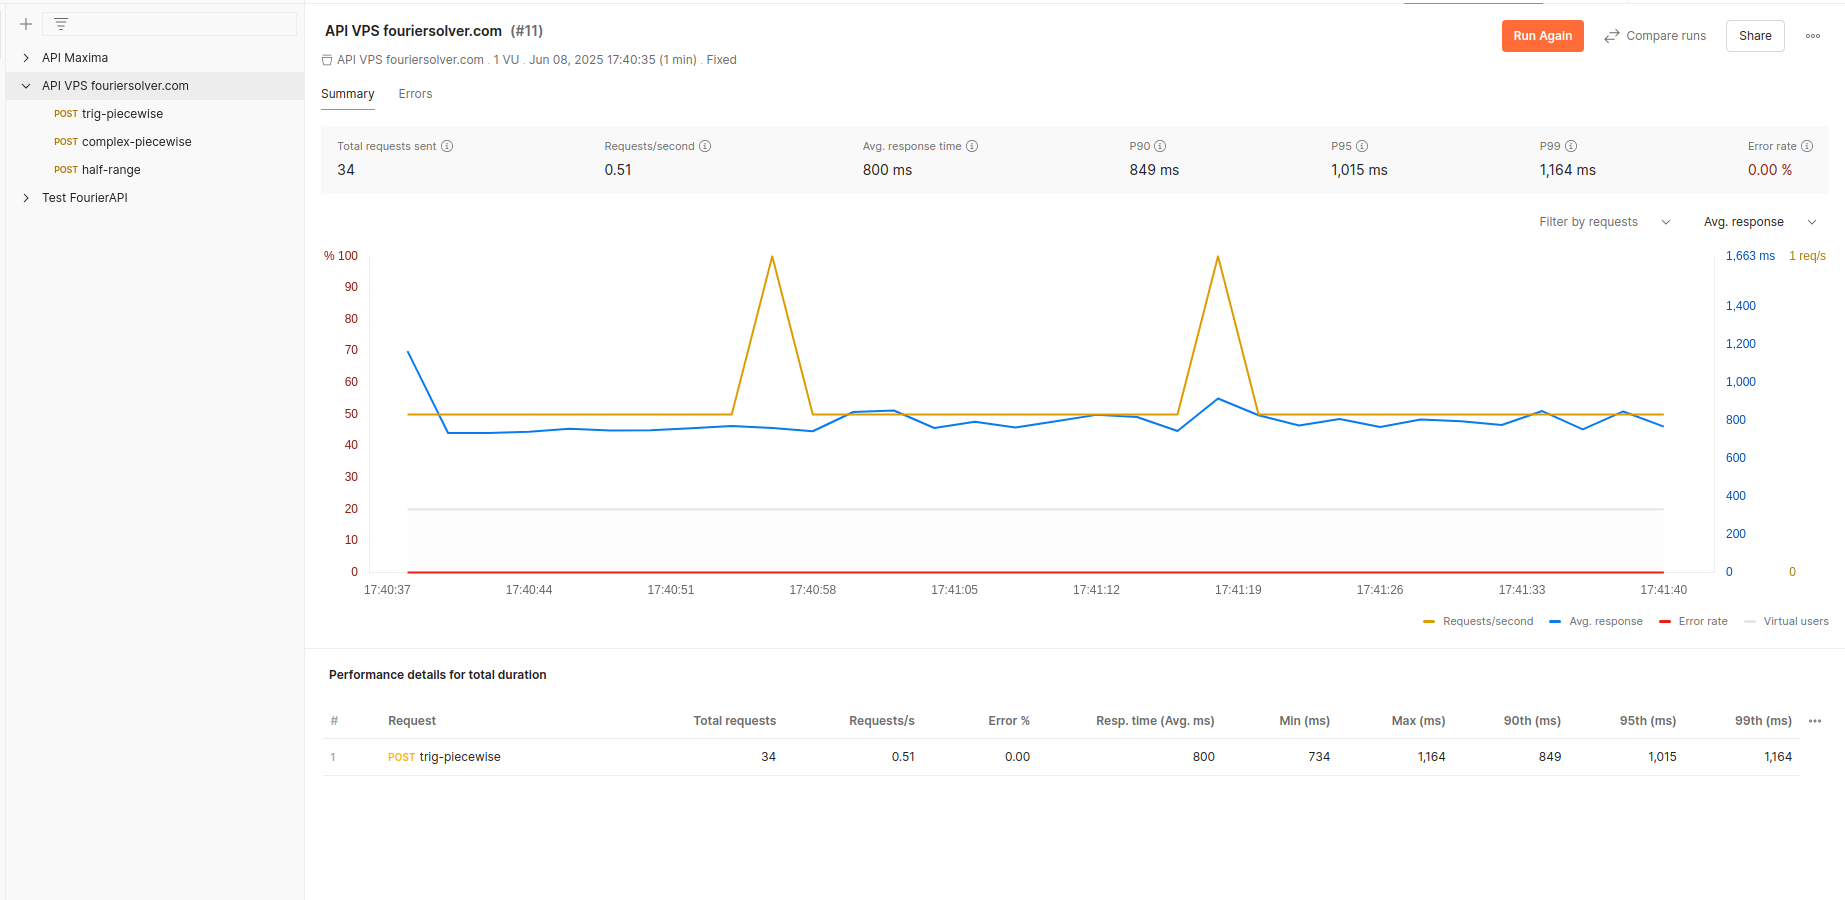
\includegraphics[width=0.95\textwidth]{img/chapter07/test-1user-trig.png}
	\caption{Prueba de rendimiento con 1 VU – Endpoint \texttt{trig-piecewise}}
	\label{fig:test-1user-trig}
\end{figure}

\begin{figure}[H]
	\centering
	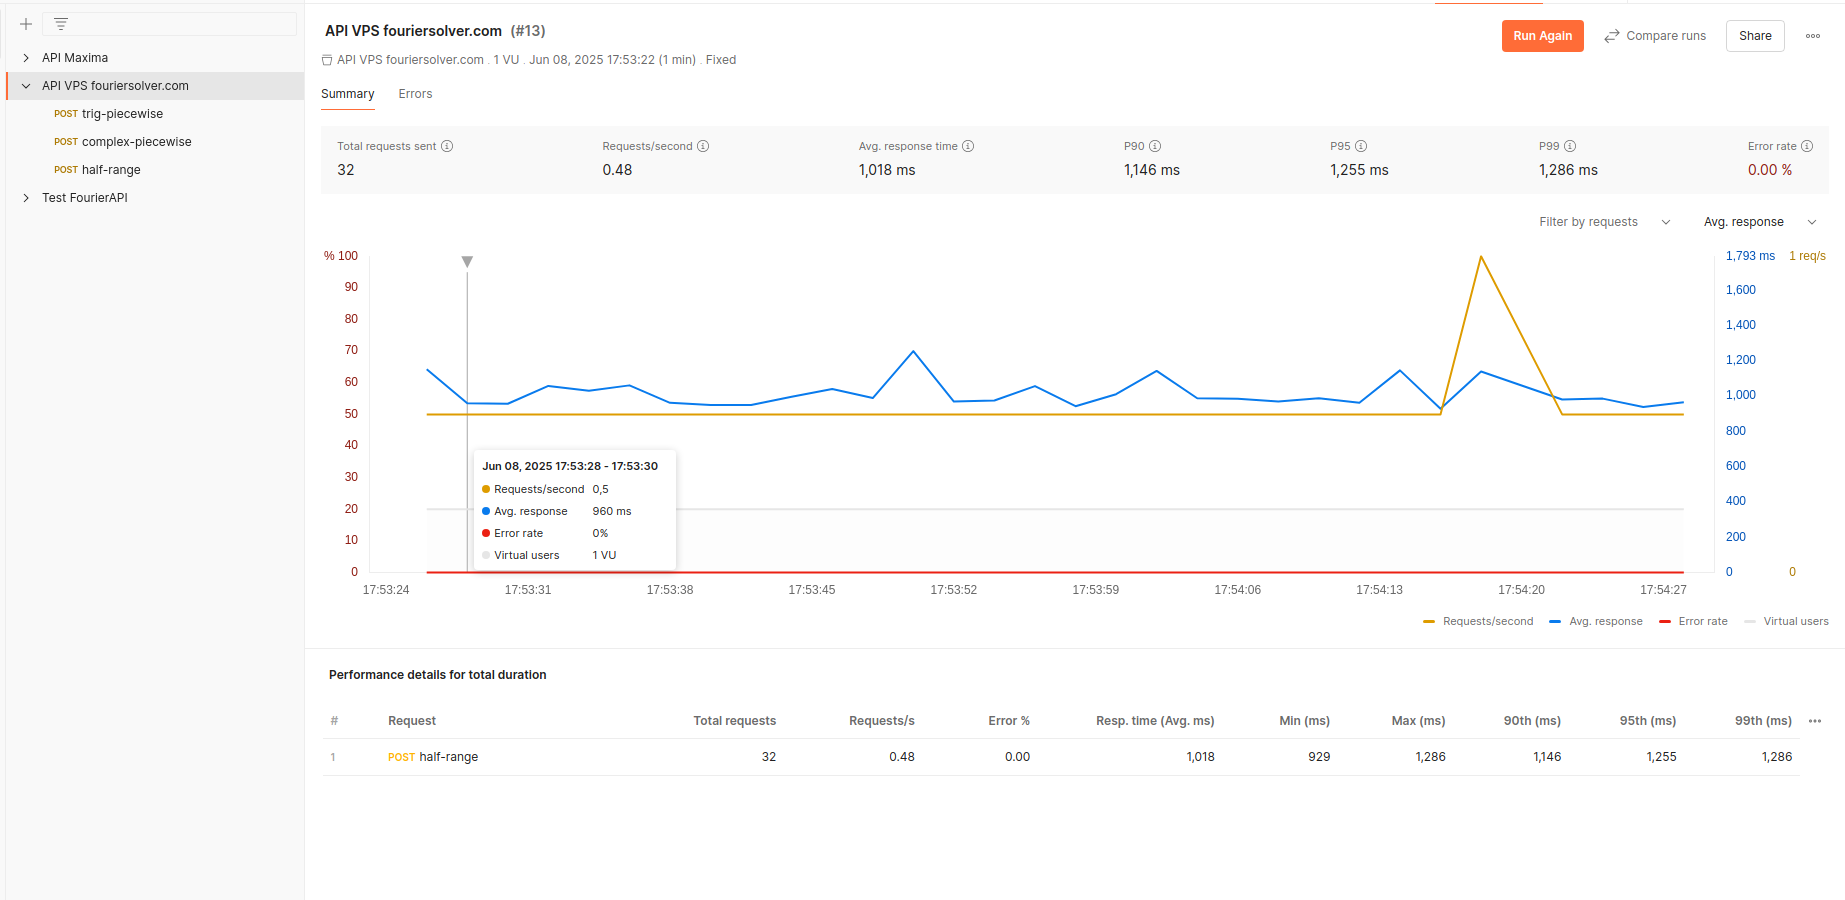
\includegraphics[width=0.95\textwidth]{img/chapter07/test-1user-half.png}
	\caption{Prueba de rendimiento con 1 VU – Endpoint \texttt{half-range}}
	\label{fig:test-1user-half}
\end{figure}

\begin{figure}[H]
	\centering
	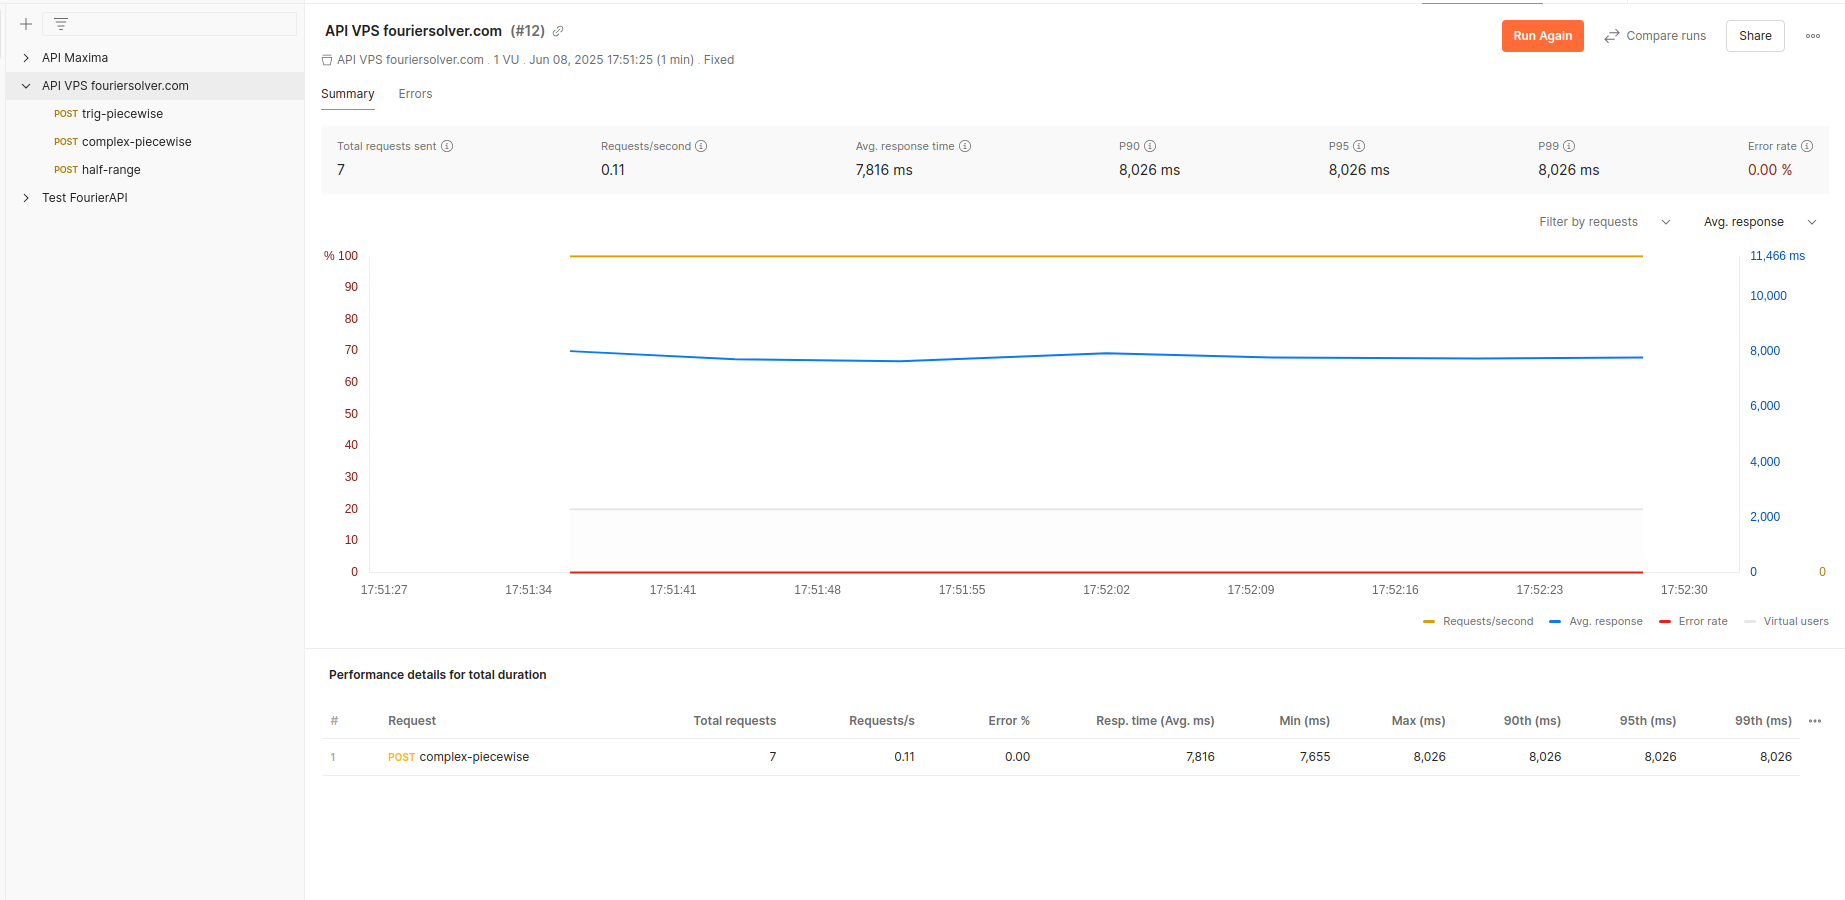
\includegraphics[width=0.95\textwidth]{img/chapter07/test-1user-complex.png}
	\caption{Prueba de rendimiento con 1 VU – Endpoint \texttt{complex-piecewise}}
	\label{fig:test-1user-complex}
\end{figure}

\begin{figure}[H]
	\centering
	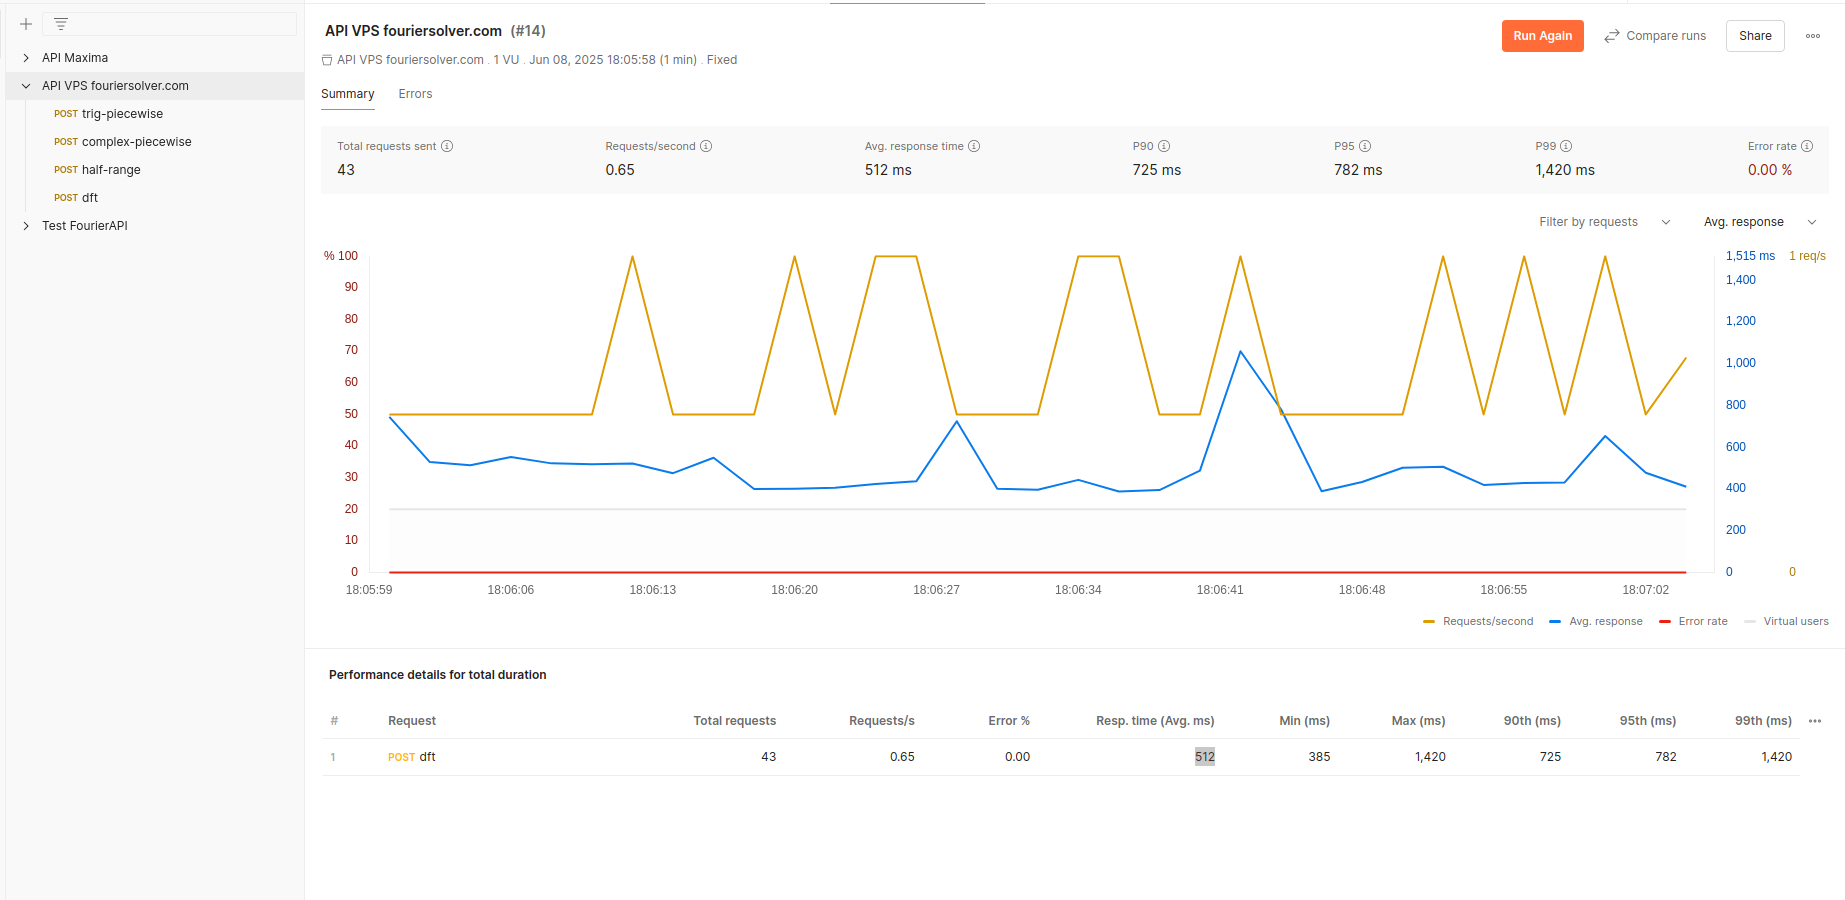
\includegraphics[width=0.95\textwidth]{img/chapter07/test-1user-dft.png}
	\caption{Prueba de rendimiento con 1 VU – Endpoint \texttt{dft}}
	\label{fig:test-1user-dft}
\end{figure}


\begin{longtable}{|m{4cm}|m{2.2cm}|m{2.2cm}|m{2.2cm}|m{2cm}|}
	\hline
	\rowcolor{black!75}
	\head{Endpoint} & \head{Prom. tiempo de respuesta (ms)} & \head{P90 (ms)} & \head{P95 (ms)} & \head{Error \%} \\ \hline
	\endfirsthead
	
	\multicolumn{5}{c}{{\tablename\ \thetable{} -- continuación}} \\
	\rowcolor{black!75}
	\head{Endpoint} & \head{Prom. tiempo de respuesta (ms)} & \head{P90 (ms)} & \head{P95 (ms)} & \head{Error \%} \\ \hline
	\endhead
	
	\hline \multicolumn{5}{r}{{Continúa en la siguiente página}} \\
	\endfoot
	
	\hline
	\endlastfoot
	
	\texttt{/trig-piecewise} & 800 & 849 & 1015 & 0.00 \\ \hline
	\texttt{/complex-piecewise} & 7816 & 8026 & 8026 & 0.00 \\ \hline
	\texttt{/half-range} & 1018 & 1146 & 1255 & 0.00 \\ \hline
	\texttt{/dft} & 512 & 725 & 782 & 0.00 \\ \hline
	
\end{longtable}
\caption{Resultados de rendimiento con 1 usuario virtual (1 VU)} \label{tabla:rendimiento-1vu}

\vspace{0.5em}

%------------- 20 VU FIGURAS ------------------------------------------------
\paragraph*{Carga moderada (20 VU)}

\begin{figure}[H]
	\centering
	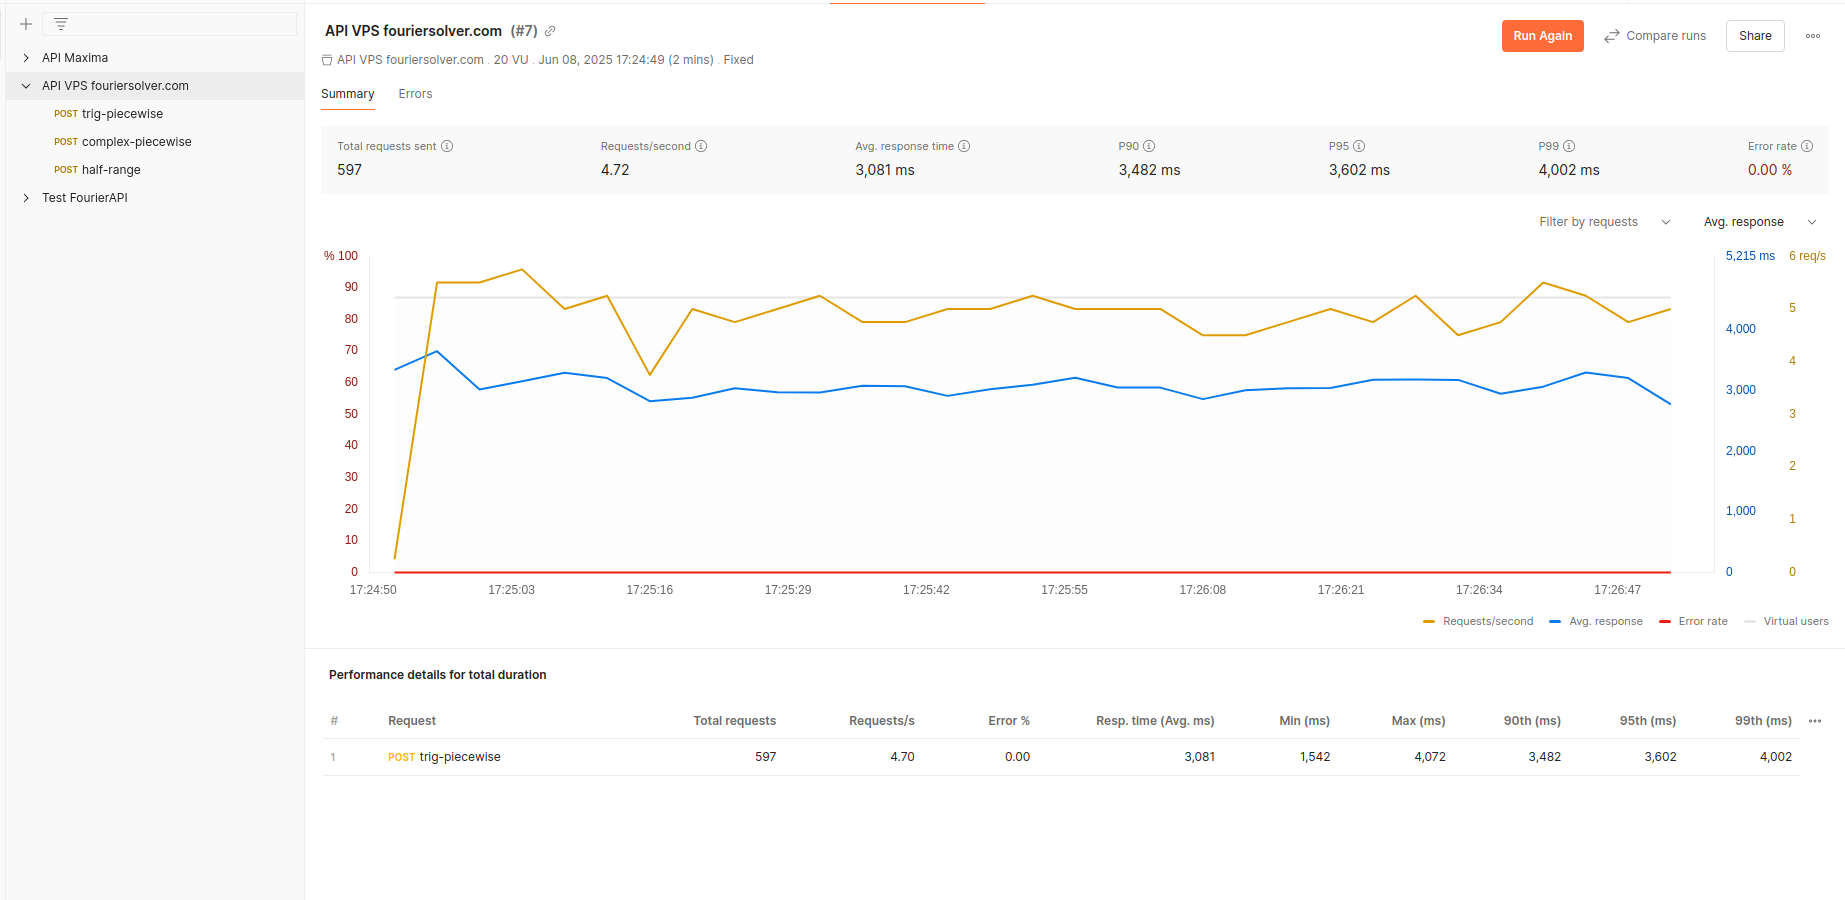
\includegraphics[width=0.95\textwidth]{img/chapter07/test-20users-trig.png}
	\caption{Prueba de rendimiento con 20 VU – Endpoint \texttt{trig-piecewise}}
	\label{fig:test-20users-trig}
\end{figure}

\begin{figure}[H]
	\centering
	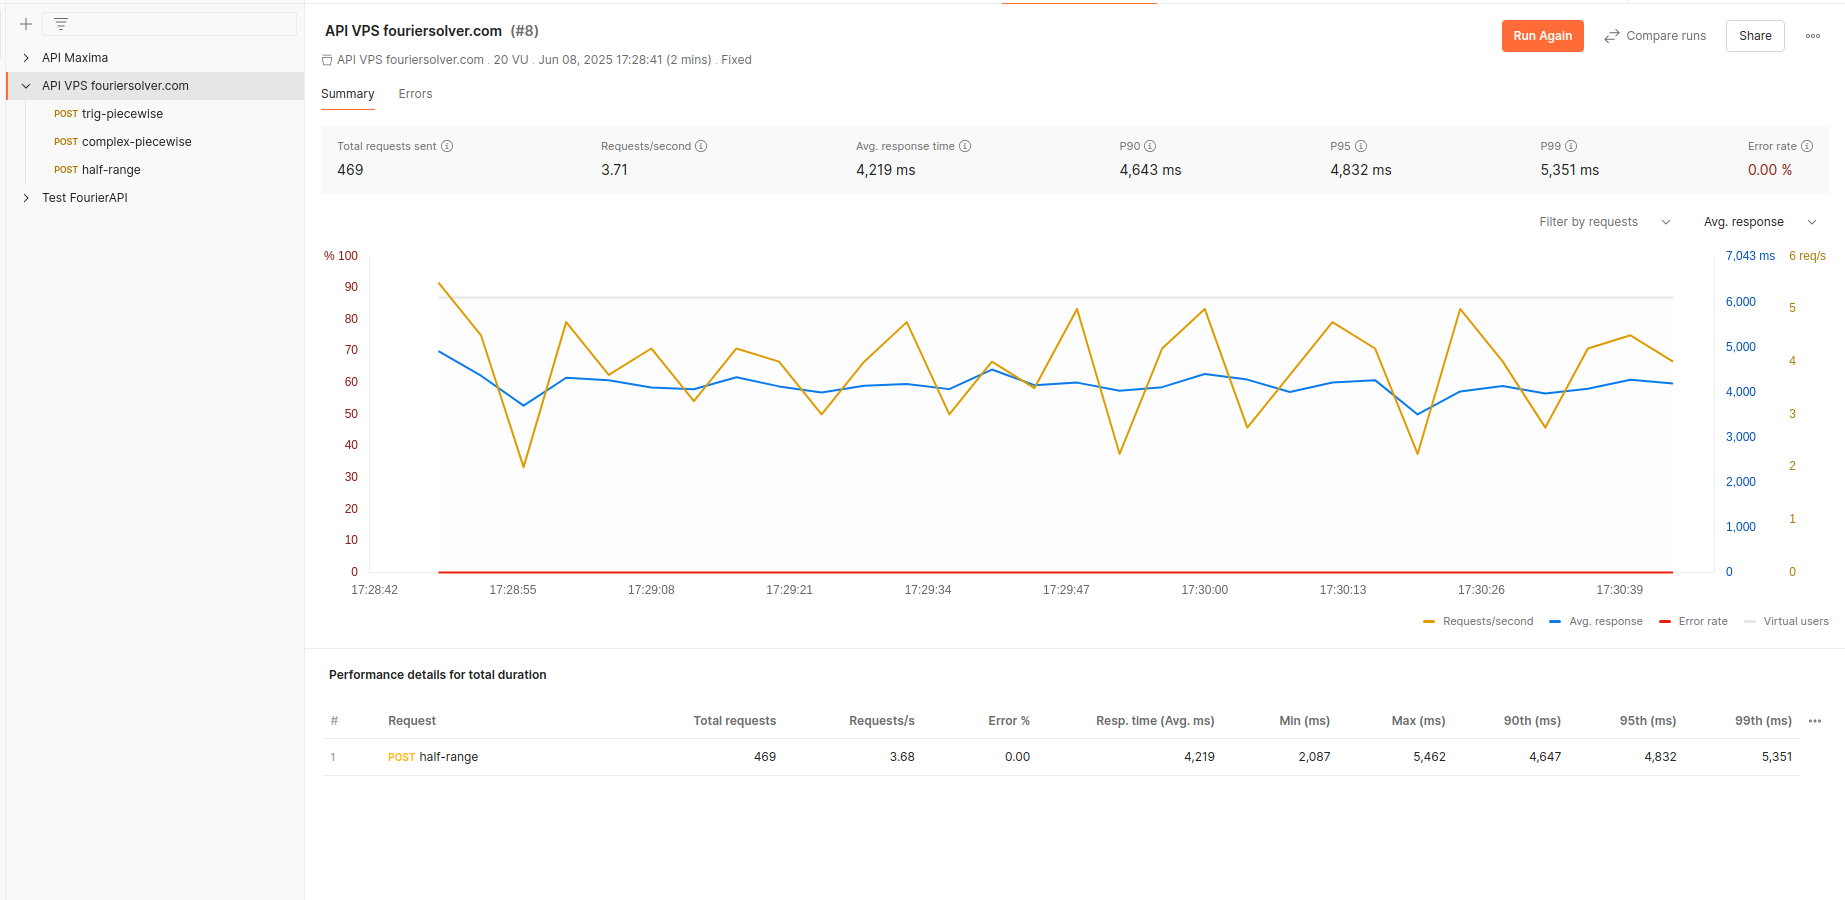
\includegraphics[width=0.95\textwidth]{img/chapter07/test-20users-half.png}
	\caption{Prueba de rendimiento con 20 VU – Endpoint \texttt{half-range}}
	\label{fig:test-20users-half}
\end{figure}

\begin{figure}[H]
	\centering
	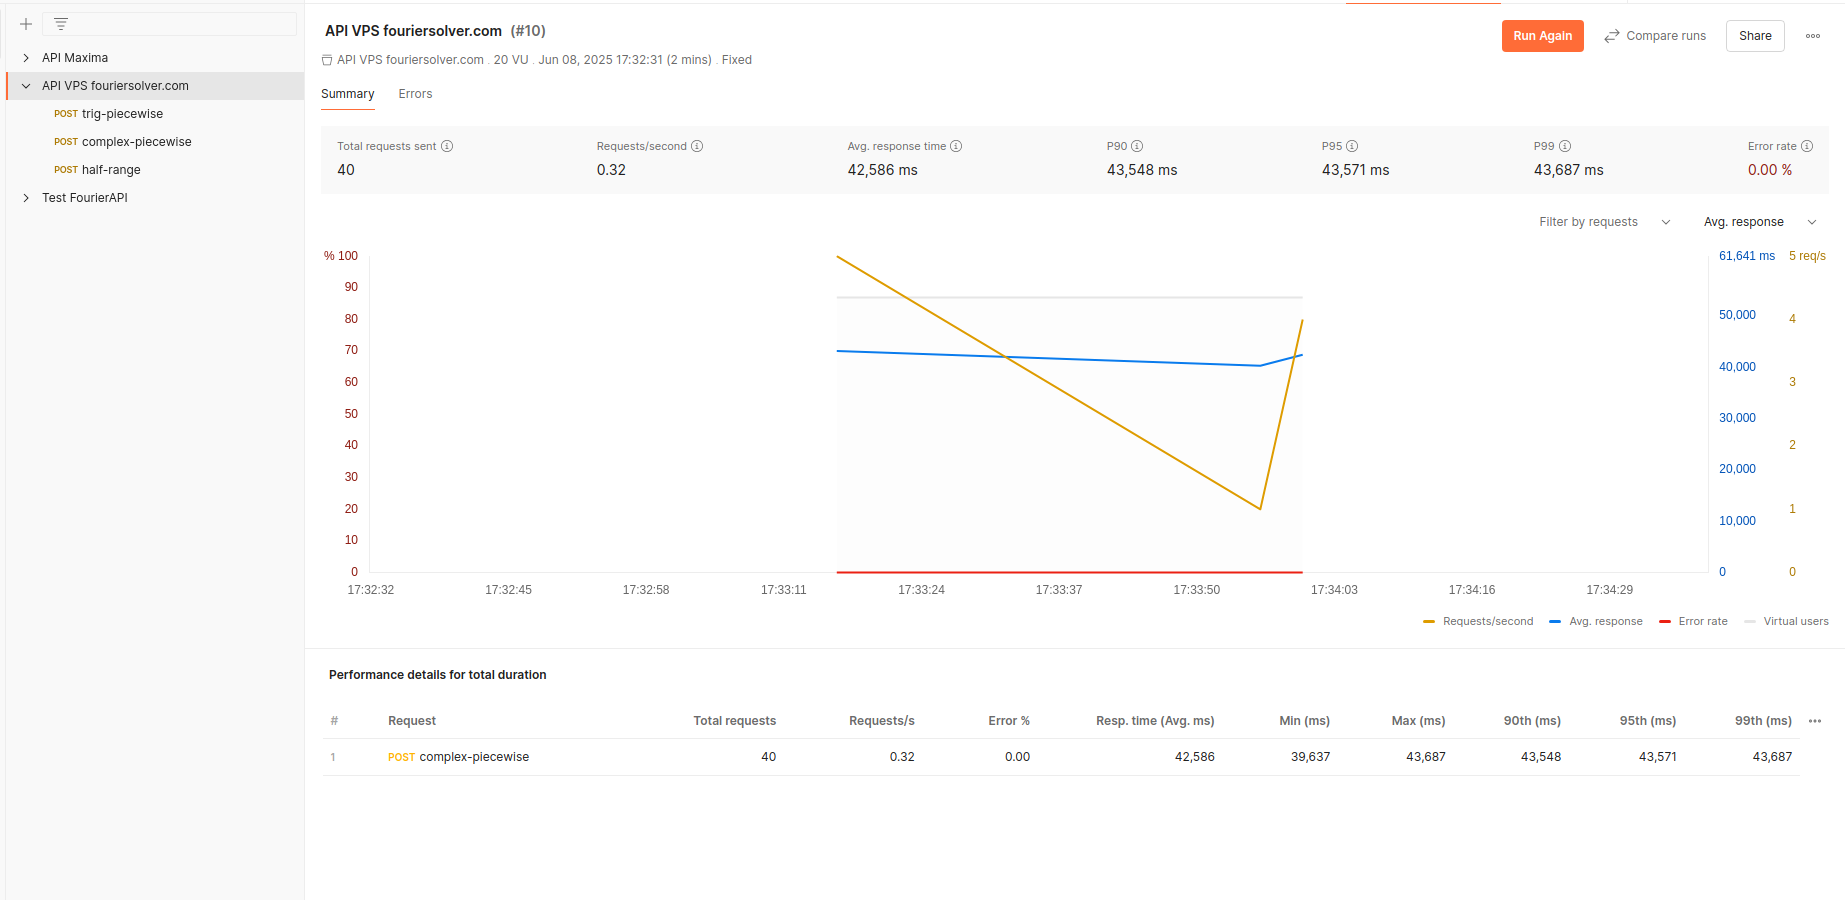
\includegraphics[width=0.95\textwidth]{img/chapter07/test-20users-complex.png}
	\caption{Prueba de rendimiento con 20 VU – Endpoint \texttt{complex-piecewise}}
	\label{fig:test-20users-complex}
\end{figure}

\begin{figure}[H]
	\centering
	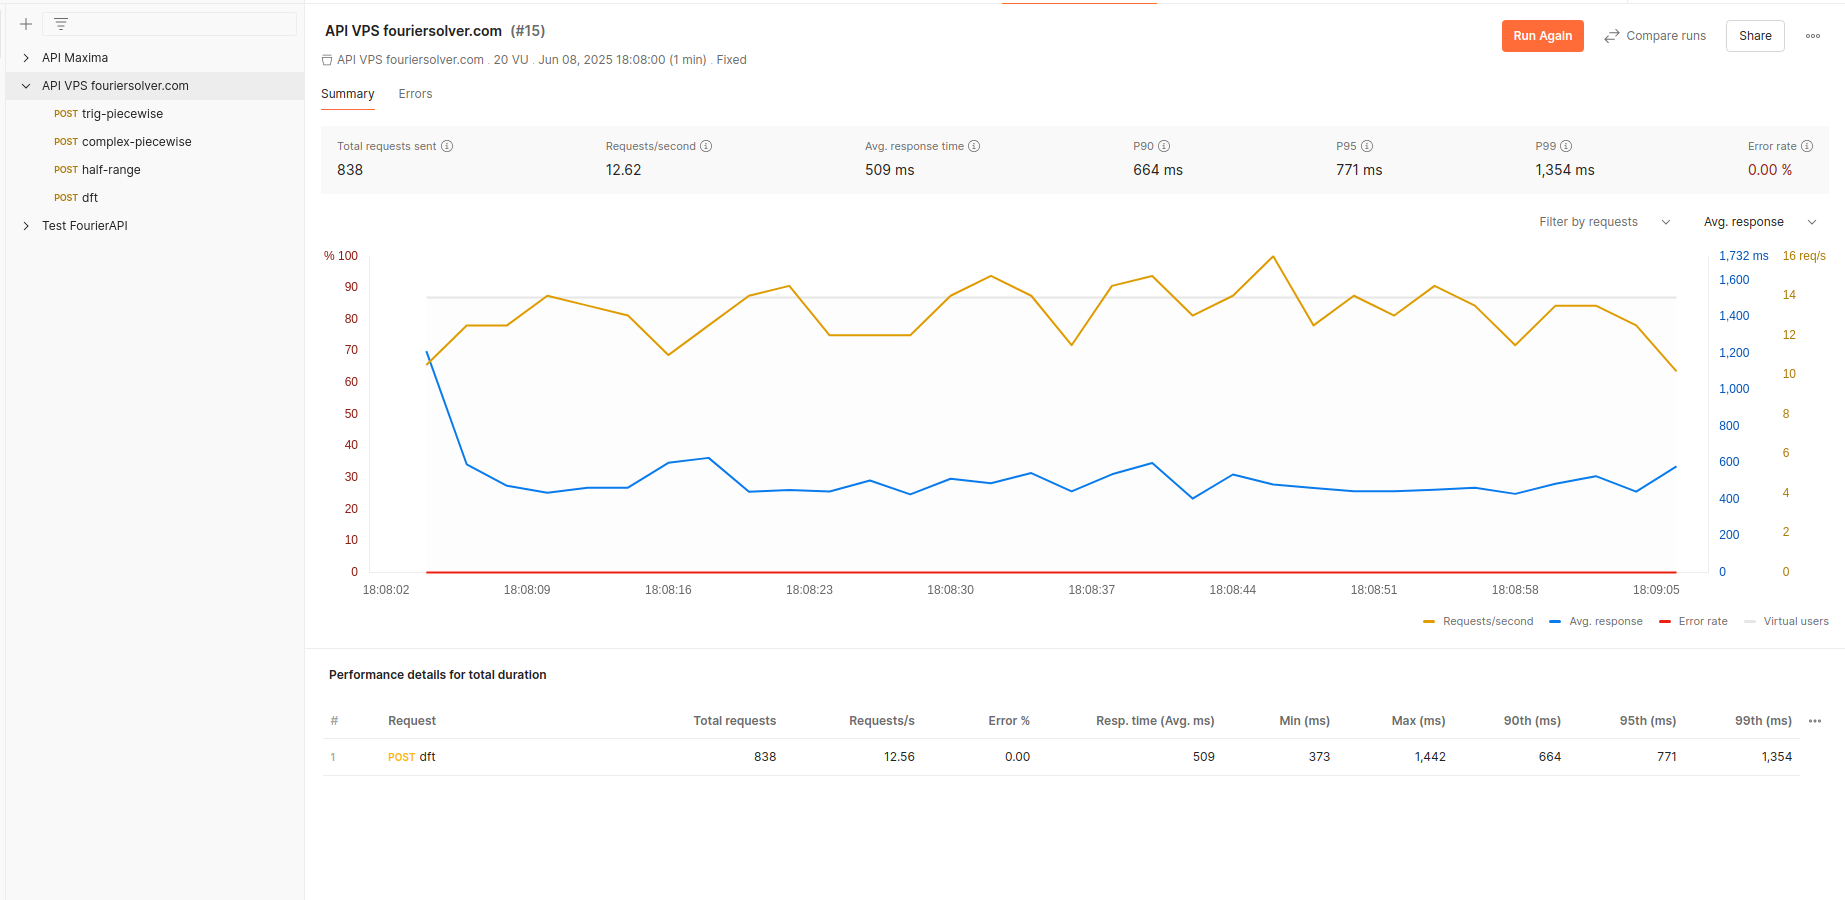
\includegraphics[width=0.95\textwidth]{img/chapter07/test-20users-dft.png}
	\caption{Prueba de rendimiento con 20 VU – Endpoint \texttt{dft}}
	\label{fig:test-20users-dft}
\end{figure}

\begin{longtable}{|m{4cm}|m{2.2cm}|m{2.2cm}|m{2.2cm}|m{2cm}|}
	\hline
	\rowcolor{black!75}
	\head{Endpoint} & \head{Prom. tiempo de respuesta (ms)} & \head{P90 (ms)} & \head{P95 (ms)} & \head{Error \%} \\ \hline
	\endfirsthead
	
	\multicolumn{5}{c}{{\tablename\ \thetable{} -- continuación}} \\
	\rowcolor{black!75}
	\head{Endpoint} & \head{Prom. tiempo de respuesta (ms)} & \head{P90 (ms)} & \head{P95 (ms)} & \head{Error \%} \\ \hline
	\endhead
	
	\hline \multicolumn{5}{r}{{Continúa en la siguiente página}} \\
	\endfoot
	
	\hline
	\endlastfoot
	
	\texttt{/trig-piecewise} & 3081 & 3482 & 3602 & 0.00 \\ \hline
	\texttt{/complex-piecewise} & 42586 & 43548 & 43571 & 0.00 \\ \hline
	\texttt{/half-range} & 4219 & 4643 & 4832 & 0.00 \\ \hline
	\texttt{/dft} & 509 & 664 & 771 & 0.00 \\ \hline
	
\end{longtable}
\caption{Resultados de rendimiento con 20 usuarios virtuales (20 VU)} \label{tabla:rendimiento-20vu}


\subsubsection*{Análisis y discusión}
Los resultados muestran un comportamiento estable sin errores HTTP incluso bajo
20 usuarios concurrentes; sin embargo, existen diferencias significativas entre
endpoints:

\begin{itemize}
	\item \textbf{Eficiencia}: El endpoint \texttt{/dft} mantiene tiempos medios
	inferiores a 600 ms incluso a 20 VU, gracias a su implementación vectorizada
	y al uso de estructuras de datos in-memory.
	\item \textbf{Cuello de botella}: \texttt{/complex-piecewise} presenta
	un incremento de casi \SI{445}{\percent} en el tiempo medio al pasar de 1
	a 20 VU, revelando que el cálculo simbólico involucrado no escala linealmente.
	\item \textbf{Endpoints trig‐ y half-range}: Aunque el tiempo medio se
	multiplica por $\sim$4–5 al aumentar la concurrencia, se mantiene por debajo
	de 5 s, valor aceptable para un servicio con procesamiento matemático intenso.
\end{itemize}

La API cumple con el SLA de \SI{95}{\percent} de respuestas por debajo de
\SI{5}{\second} para tres de los cuatro endpoints probados incluso con 20 VU.
El endpoint \texttt{/complex-piecewise} requiere optimización—por ejemplo,
estrategias de \textit{memoization}, paralelización del cálculo simbólico o
externalización a un micro-servicio especializado—antes de un despliegue a
producción con cargas elevadas.

%----------------------------------------------------------------------------------------

\subsection{Pruebas con Usuarios Finales}
Se realizaron pruebas con estudiantes para validar la usabilidad y utilidad del sistema en contextos educativos. Se documentan los escenarios de prueba y el feedback recibido.

%======================================================================
\section{Análisis de Complejidad Computacional}
%======================================================================

Esta sección cuantifica rigurosamente el costo temporal y espacial de los
dos algoritmos implementados en el sistema para estudiar funciones
periódicas:

\begin{itemize}
	\item \textbf{Método simbólico}: cálculo exacto de coeficientes de
	Fourier mediante integración (con detección de
	indeterminaciones).
	\item \textbf{Método numérico}: Transformada Discreta de Fourier (DFT)
	sobre un conjunto finito de muestras y recreación de la señal
	periódica.
\end{itemize}

%----------------------------------------------------------------------
\subsection{Complejidad Temporal}
%----------------------------------------------------------------------

El tiempo de ejecución se desglosa por componentes funcionales:

\begin{enumerate}
	\item \textbf{Cálculo simbólico de coeficientes}: 
	$O(m \cdot c)$, siendo  
	$m$ el número de tramos de la función definida por partes y  
	$c$ la complejidad de la integración simbólica de un tramo.
	
	\item \textbf{Evaluación numérica de $2N + 1$ coeficientes} (serie
	\textit{compleja}): $O(N \cdot m \cdot c)$.
	
	\item \textbf{Detección de indeterminaciones}:  
	$O(s \cdot m \cdot c)$, donde $s$ es el número de singularidades
	potenciales detectadas.
	
	\item \textbf{Resolución de límites} en los puntos singulares:  
	$O(s \cdot m \cdot c)$.
\end{enumerate}

\noindent\textbf{Cota temporal total}:

\[
T(m,N,s,c)=O\!\bigl((N+s)\,m\,c\bigr)
\]

En la configuración habitual ($N=100$ y $s\ll N$),
la complejidad efectiva se aproxima a  
$O(m\,c)$, es decir, crece linealmente con el número de tramos.

%----------------------------------------------------------------------
\subsection{Complejidad Espacial}
%----------------------------------------------------------------------

El consumo de memoria se distribuye en tres estructuras principales:

\begin{enumerate}
	\item \textbf{Expresiones simbólicas}: $O(m \cdot e)$, donde
	$e$ es el tamaño medio (en nodos del AST) de cada expresión.
	\item \textbf{Coeficientes numéricos}:  
	$O(N)$ para series trigonométricas y $O(2N+1)$ para series complejas.
	\item \textbf{Términos de la serie}: $O(N_{\text{términos}})$, con
	$N_{\text{términos}}=100$ en la práctica.
\end{enumerate}

\[
S(m,e,N)=O\!\bigl(m\,e+N\bigr)
\]

%----------------------------------------------------------------------
\subsection{Factores de Optimización}
%----------------------------------------------------------------------

El sistema incorpora estrategias específicas para mitigar el costo
computacional:

\begin{itemize}
	\item \textbf{Reutilización de resultados simbólicos}.  
	Los coeficientes previamente calculados se aprovechan para
	detectar y resolver indeterminaciones sin reintegrar.
	\item \textbf{Paralelización implícita}.  
	La resolución de límites se ejecuta con \texttt{Promise.all},
	permitiendo la explotación de hilos de trabajo en \textit{Node.js}.
	\item \textbf{Simplificación adaptativa}.  
	Se aplican diferentes niveles de simplificación según el tipo de
	serie (trigonométrica o compleja) y el tamaño de la expresión.
\end{itemize}

 \subsection{Análisis de la Función \texttt{findIndeterminateValues} y Cálculo de Límites}
%======================================================================
\section{Detección de Indeterminaciones y Cálculo de Límites}
%======================================================================

Una parte crítica del proceso de generación de coeficientes para series
de Fourier es la detección de singularidades que impiden evaluar
simbólicamente ciertos términos.  
Para ello, el sistema implementa una función específica denominada
\texttt{findIndeterminateValues}, cuya complejidad se analiza a
continuación.

\subsection{Entrada estructurada}

La entrada del algoritmo se organiza como una matriz
\texttt{funcionMatrix} de tamaño \( p \times 3 \), donde cada fila tiene
la forma \([f(x), a, b]\) y representa un tramo definido por partes de la
función a analizar.  

Cada expresión \( f(x) \) puede contener operadores racionales,
trigonométricos, exponenciales o funciones definidas a trozos.

\subsection{Fase de detección y resolución}

El procedimiento interno de \texttt{findIndeterminateValues} consiste en:

\begin{enumerate}
	\item Calcular simbólicamente los coeficientes sin asumir que \( n \in \mathbb{Z} \).
	\item Extraer el denominador de cada expresión dependiente de \( n \).
	\item Resolver \( \text{denom}(n) = 0 \) para encontrar posibles valores
	indeterminados.
	\item Para cada raíz encontrada, calcular el límite correspondiente.
\end{enumerate}

La complejidad temporal está dada por:

\[
T_{\text{indet}} = O\left(p \cdot T_{\text{int}}^{(f)} + S \cdot T_{\text{lim}}^{(f)}\right)
\]

donde:
\begin{itemize}
	\item \( p \): número de tramos.
	\item \( T_{\text{int}}^{(f)} \): costo de integrar \( f(x) \) sin asumir \( n \in \mathbb{Z} \).
	\item \( S \): número de singularidades detectadas.
	\item \( T_{\text{lim}}^{(f)} \): costo de evaluar el límite en una raíz.
\end{itemize}

%----------------------------------------------------------------------
\subsection{Complejidad de la función \texttt{limit} en Maxima}
%----------------------------------------------------------------------

\begin{longtable}{|c|m{4cm}|m{3.5cm}|m{3.3cm}|m{3cm}|}
	\hline
	\rowcolor{black!75}
	\head{\#} & \head{Método / Ruta en \texttt{limit}} & \head{Cuándo se aplica} & \head{Pasos dominantes} & \head{Complejidad} \\ \hline
	\endfirsthead
	\multicolumn{5}{c}{{\tablename\ \thetable{} -- continuación}} \\ \hline
	\rowcolor{black!75}
	\head{\#} & \head{Método / Ruta en \texttt{limit}} & \head{Cuándo se aplica} & \head{Pasos dominantes} & \head{Complejidad} \\ \hline
	\endhead
	\hline \multicolumn{5}{r}{{Continúa en la siguiente página}} \\ \hline
	\endfoot
	\hline
	\endlastfoot
	
	1 & Reglas heurísticas y tablas & Funciones elementales típicas & Recorrido del árbol de sintaxis & \( O(n) \) \\ \hline
	2 & Cambio de variable automático & Patrones tipo \( f(g(x))g'(x) \) & Sustituciones recursivas & \( O(n^2) \) \\ \hline
	3 & Reescritura algebraica & Productos y cocientes simplificables & Aplicación de identidades & \( O(n^2) \) \\ \hline
	4 & Regla de L’Hôpital & Indeterminaciones tipo \( 0/0 \), \( \infty/\infty \) & Derivación sucesiva & \( O(n) \) \\ \hline
	5 & Expansión en series (Taylor) & Límite no directo & Expansión + evaluación & \( O(n^2) \) \\ \hline
	6 & Método de Gruntz & Funciones con comportamiento oscilante o exponencial & Análisis asintótico & \( O(n^2) \) \\ \hline
	7 & Sustituciones simbólicas & Expresiones racionales o trigonométricas simples & Simplificación previa al cálculo & \( O(n) \) \\ \hline
	
\end{longtable}
\caption{Complejidad de los métodos usados por \texttt{limit} en Maxima}
\label{tabla:limit-complejidad}

\vspace{0.5cm}

%----------------------------------------------------------------------
\subsection{Impacto en la complejidad global}
%----------------------------------------------------------------------

Incluir una fase de detección de indeterminaciones y cálculo de límites
modifica la complejidad total del sistema, particularmente en funciones con
alto grado de simbolismo.

La nueva expresión asintótica queda como:

\[
T_{\text{total}} =
O\left(p \cdot T_{\text{int}}^{(f)} + S \cdot T_{\text{lim}}^{(f)} + N \cdot P^2\right)
\]

Donde:
\begin{itemize}
	\item El primer término representa las integraciones sin $n$ entero.
	\item El segundo término corresponde a la resolución de indeterminaciones.
	\item El tercero, al cálculo de los coeficientes para cada valor de $n$.
\end{itemize}

En casos reales, el número de singularidades $S$ es bajo, y $T_{\text{lim}}^{(f)}$
suele resolverse en tiempo polinomial, por lo que el impacto en rendimiento es
contenible y no dominante en la mayoría de los escenarios.


%======================================================================
\section{Casos Especiales y Robustez}
%======================================================================

El algoritmo contempla circunstancias excepcionales para garantizar
confiabilidad operativa:

\begin{enumerate}
	\item \textbf{Indeterminaciones}.  
	Se resuelven mediante cálculo de límites simbólicos o numéricos.
	\item \textbf{Errores en Maxima}.  
	Se capturan y propagan con mensajes de diagnóstico detallados.
	\item \textbf{Datos inconsistentes}.  
	La estructura de entrada se valida exhaustivamente antes de
	procesar cualquier tramo.
\end{enumerate}

%======================================================================
\section{Modelo de Complejidad de la Función \texttt{integrate}}
%======================================================================

La eficiencia global está condicionada por el costo interno de
\texttt{integrate} en Maxima.  
La \autoref{tabla:integrate-complejidad} resume sus rutas principales y
las complejidades asociadas.

\begin{longtable}{|c|m{3cm}|m{2.8cm}|m{3.2cm}|m{2.5cm}|}
	\hline
	\rowcolor{black!75}
	\head{\#} & \head{Método / Ruta} & \head{Cuándo se aplica} &
	\head{Pasos dominantes} & \head{Complejidad} \\ \hline
	\endfirsthead
	\multicolumn{5}{c}{{\tablename\ \thetable{} -- continuación}} \\ \hline
	\rowcolor{black!75}
	\head{\#} & \head{Método / Ruta} & \head{Cuándo se aplica} &
	\head{Pasos dominantes} & \head{Complejidad} \\ \hline
	\endhead
	\hline \multicolumn{5}{r}{{Continúa en la siguiente página}} \\ \hline
	\endfoot
	\hline
	\endlastfoot
	1 & Reglas heurísticas
	& Funciones elementales típicas
	& Recorrido del AST
	& $O(n)$ \\ \hline
	2 & Cambio de variable automático
	& Patrones $f(g(x))g'(x)$
	& Sustituciones recursivas
	& $O(n^2)$ \\ \hline
	3 & Integración por partes heurística
	& Productos $u\,v'$
	& Combinaciones $u,v$
	& $O(n^2)$ \\ \hline
	4 & Hermite / racional
	& Cocientes $P/Q$
	& Descomposición + álgebra lineal
	& $O(d^3)$ \\ \hline
	5 & Fracciones parciales / residuos
	& Racionales factorizables
	& Sistemas lineales
	& $O(d^3)$ \\ \hline
	6 & Risch--Norman (rápido)
	& $\exp$, $\log$ sencillos
	& Álgebra estructural
	& $O(2^k)$ \\ \hline
	7 & Risch completo
	& Funciones elementales arbitrarias
	& Torres de extensiones
	& $O(2^{2^k})$ \\ \hline
	8 & Funciones especiales
	& $\Gamma$, $\mathrm{erf}$, etc.
	& Patrón directo
	& $O(n)$ \\ \hline
	9 & Integral definida simbólica
	& $\int_a^b f(x)\,dx$
	& Indefinida $+$ límites
	& $O(T_{\text{indef}})+O(n)$ \\ \hline
	10 & Análisis complejo
	& Racionales con polos
	& Cálculo de residuos
	& $O(d^3)$ \\ \hline
\end{longtable}
\caption{Complejidad de los métodos internos de \texttt{integrate} (sin fuentes).}
\label{tabla:integrate-complejidad-sin-fuente}


\vspace{0.5cm}

%======================================================================
\section{Modelo Asintótico del Sistema}
%======================================================================

\subsection{Descomposición por etapas}

\begin{longtable}{|c|m{4.5cm}|m{2.5cm}|m{3.2cm}|m{2.8cm}|}
	\hline
	\rowcolor{black!75}
	\head{Paso} & \head{Qué hace} & \head{\# veces} &
	\head{Dominante} & \head{Complejidad} \\ \hline
	\endfirsthead
	\multicolumn{5}{c}{{\tablename\ \thetable{} -- continuación}} \\ \hline
	\rowcolor{black!75}
	\head{Paso} & \head{Qué hace} & \head{\# veces} &
	\head{Dominante} & \head{Complejidad} \\ \hline
	\endhead
	\hline \multicolumn{5}{r}{{Continúa en la siguiente página}} \\ \hline
	\endfoot
	\hline
	\endlastfoot
	1 & Normalización inicial
	& 1
	& Lectura de $M$ filas
	& $O(M)$ \\ \hline
	2 & Coeficientes sin $n\in\mathbb{Z}$
	& $M$
	& $M$ integrales
	& $O(M\,I(P))$ \\ \hline
	3 & Detección de indeterminaciones
	& $\le M$
	& Factorización $+$ límites
	& $O(P^3+s\,I(P))$ \\ \hline
	4 & Cálculo con $n\in\mathbb{Z}$ ($2N{+}1$)
	& $2N+1$
	& Sustituciones $+$ simplif.
	& $O(N\,P^2)$ \\ \hline
	5 & Amplitud, fase y términos
	& $2N+1$
	& Álgebra básica
	& $O(N)$ \\ \hline
	6 & Ensamblado final
	& 1
	& Serialización JSON
	& $O(M+N)$ \\ \hline
\end{longtable}
\caption{Complejidad por fases del algoritmo.}
\label{tabla:fases-algoritmo}

\subsection{Complejidad total}

El tiempo total se aproxima a

\[
T_{\text{total}} =
O\!\bigl((M+s)\,I(P)+N\,P^2\bigr),
\]

\noindent donde $I(P)$ es la complejidad del método de integración
seleccionado por Maxima.  
En el peor caso, si se activa el algoritmo de Risch completo:

\[
I(P)=O(2^{2^{P}}) \quad\Longrightarrow\quad
T_{\text{total}}=O\!\bigl((M+s)\,2^{2^{P}}+N\,P^2\bigr).
\]

Sin embargo, en la práctica Maxima recurre mayoritariamente a heurísticas
$O(P)$ o métodos racionales $O(P^3)$, por lo que el tiempo real permanece
muy por debajo de la cota teórica.

\subsection{Complejidad espacial}

El uso de memoria está acotado por

\[
S_{\text{total}}=O\!\bigl(M\,P+N\bigr),
\]

\noindent el cual contempla tanto las estructuras simbólicas intermedias
como las listas de coeficientes y términos gráficos.  
La serialización intermedia (JSON, \LaTeX) no altera el orden de
magnitud.

%======================================================================
%----------------------------------------------------------------------
\subsection{Complejidad Temporal (DFT)}
%----------------------------------------------------------------------

El procedimiento numérico basado en la Transformada Discreta de Fourier
se descompone en cuatro fases principales:

\begin{enumerate}
	\item \textbf{Evaluación puntual} de la función en $N$ muestras: 
	$O\bigl(N \, M_{f}\bigr)$, donde $M_{f}$ es el costo de evaluar la
	función por tramos en un punto (típicamente $O(1)$ si sólo hay
	operaciones elementales).
	\item \textbf{Cálculo de la DFT} mediante FFT: 
	$O\bigl(N \log N\bigr)$.
	\item \textbf{Reconstrucción periódica} de la señal (extensión a
	$2M{+}1$ períodos para visualización o convolución): 
	$O\bigl(N \, M\bigr)$.
	\item \textbf{Extracción de espectros} (módulo y argumento de cada
	coeficiente): $O(N)$.
\end{enumerate}

\[
\boxed{\;
	T_{\text{DFT}}
	= O\!\bigl(N \, M_{f} + N \log N + N \, M\bigr)
	\;}
\]

Bajo el supuesto habitual de $M_{f}=O(1)$ y un número moderado de
períodos extra ($M=O(1)$), la cota se simplifica a

\[
T_{\text{DFT}} = O\!\bigl(N \log N\bigr).
\]

%----------------------------------------------------------------------
\subsection{Complejidad Espacial (DFT)}
%----------------------------------------------------------------------

Los recursos de memoria se reparten en:

\begin{itemize}
	\item \textbf{Muestras originales}: $N$ pares $(x_k,\,f(x_k))$.
	\item \textbf{Coeficientes complejos}: $N$ valores $F_k$.
	\item \textbf{Amplitudes y fases}: $N$ magnitudes y argumentos.
	\item \textbf{Señal reconstruida}: $(2M+1)\,N$ puntos para los $M$
	períodos adicionales a cada lado.
\end{itemize}

\[
\boxed{\;
	S_{\text{DFT}}
	= O\!\bigl(N \,(M + 3)\bigr)
	= O\!\bigl(N\,M\bigr)
	\;}
\]

En la práctica, cuando la reconstrucción periódica no se almacena
completa (p.\,ej.\ se genera en streaming), el requerimiento dominante
baja a $O(N)$.

